% The Critical Line Algorithm as implemented in cvxcla
%
% This paper documents the algorithm implemented in src/cvxcla/cla.py
% (with supporting modules first.py, operators.py and types.py).
%
% JSS submission. Build with:
%   pdflatex cla.tex; bibtex cla; pdflatex cla.tex; pdflatex cla.tex
% The class/style files jss.cls, jss.bst and jsslogo.jpg are vendored under
% cls/jss/ (they are not on CTAN / in TeX Live; the journal distributes them);
% the shared Makefile puts that folder on TEXINPUTS/BSTINPUTS, so a plain `make
% pdf` is the reliable way to build this file.
% Drafting uses the [nojss] option to suppress the journal masthead; drop it for
% the final camera-ready submission.

\documentclass[article,nojss]{jss}

%% --- packages not already loaded by jss.cls --------------------------------
%% jss.cls provides: graphicx, xcolor, fancyvrb, fontenc(T1), upquote, lmodern,
%% hyperref and natbib(authoryear,round). Do NOT reload those.
\usepackage{amsmath, amssymb}
\usepackage{amsthm}
\usepackage{tikz}
\usetikzlibrary{positioning,arrows.meta}
\newtheorem{proposition}{Proposition}
\usepackage{bm}
\usepackage{booktabs}
\usepackage{array}
\usepackage{listings}

\graphicspath{{figures/}}
\raggedbottom % unbreakable code boxes leave short pages, not stretched gaps

% Code input (Python) and console output styles for the usage section. xcolor is
% supplied by jss.cls, so the colour-mixing syntax below is available.
\definecolor{codebg}{RGB}{255,252,228}   % very mild yellow
\lstdefinestyle{pyin}{%
  language=Python,
  basicstyle=\ttfamily\small,
  keywordstyle=\color{blue!50!black},
  commentstyle=\color{green!45!black}\itshape,
  stringstyle=\color{purple!60!black},
  showstringspaces=false,
  breaklines=true,
  frame=single,
  rulecolor=\color{black!25},
  backgroundcolor=\color{codebg},
  framesep=4pt,
  xleftmargin=4pt,
  xrightmargin=4pt,
  columns=fixed,
  basewidth=0.525em,
  keepspaces=true,
  aboveskip=6pt,
  belowskip=6pt,
}
\lstdefinestyle{pyout}{%
  basicstyle=\ttfamily\small\color{black!75},
  frame=single,
  rulecolor=\color{black!15},
  backgroundcolor=\color{black!3},
  framesep=4pt,
  xleftmargin=4pt,
  xrightmargin=4pt,
  breaklines=true,
  columns=fixed,
  basewidth=0.525em,
  keepspaces=true,
  aboveskip=6pt,
  belowskip=6pt,
}
% Typeset the JSS code environments with listings: Python input in a mild yellow
% box, console output in a light grey one.
\let\CodeInput\relax\let\endCodeInput\relax
\let\CodeOutput\relax\let\endCodeOutput\relax
\lstnewenvironment{CodeInput}{\lstset{style=pyin}}{}
\lstnewenvironment{CodeOutput}{\lstset{style=pyout}}{}

% The algorithm listing is typeset with only base LaTeX (a boxed minipage plus
% nested enumerate), so the paper builds without the algorithm/algorithmicx
% packages, which are not present in every TeX distribution.

% jss.cls defines \pkg; provide the remaining JSS markup macros only if absent.
\providecommand{\proglang}[1]{\textsf{#1}}
\providecommand{\code}[1]{\texttt{#1}}
\providecommand{\fct}[1]{\texttt{#1}}

% --- notation shortcuts -------------------------------------------------
\newcommand{\R}{\mathbb{R}}
\newcommand{\Sig}{\Sigma}
\newcommand{\F}{\mathcal{F}}        % free set
\newcommand{\B}{\mathcal{B}}        % blocked set
\newcommand{\Sset}{\mathcal{S}}     % active inequality-row set
\newcommand{\lb}{\ell}              % lower bound
\newcommand{\ub}{u}                 % upper bound
\newcommand{\trans}{^{\mathsf{T}}}
\newcommand{\inv}{^{-1}}
\DeclareMathOperator*{\argmax}{arg\,max}
\DeclareMathOperator*{\argmin}{arg\,min}

% --- repository links ---------------------------------------------------
% \srcfile{url-path}{display}: a clickable link to a file in the repository.
% The url-path uses literal underscores; the display escapes them for \texttt.
\newcommand{\repourl}{https://github.com/cvxgrp/cvxcla}
% Pin source links to an immutable commit, not the moving \texttt{main} branch,
% so they do not rot as the code is refactored. Bump \srcref to the
% tagged/archived release (the Zenodo-archived commit) at submission time.
\newcommand{\srcref}{v2.7.1}
\newcommand{\srcfile}[2]{\href{\repourl/blob/\srcref/#1}{\texttt{#2}}}
% \target{name}: one step of the reproduction script, run as
% `uv run experiments/make_figures.py name`.
\newcommand{\target}[1]{\srcfile{experiments/make_figures.py}{make\_figures.py~#1}}

%% --- JSS front matter ------------------------------------------------------
\author{Thomas Schmelzer\\Jebel Quant Research}
\Plainauthor{Thomas Schmelzer}

\title{\pkg{cvxcla}: The Critical Line Algorithm with an Operator Interface in
  \proglang{Python}}
\Plaintitle{cvxcla: The Critical Line Algorithm with an Operator Interface in Python}
\Shorttitle{\pkg{cvxcla}: The Critical Line Algorithm in \proglang{Python}}

\Abstract{
\pkg{cvxcla} is an open-source \proglang{Python} implementation of Markowitz's
Critical Line Algorithm (CLA), which returns the \emph{entire} mean--variance efficient
frontier as a finite list of turning points, with no discretisation error. The turning
points are Markowitz's; the package adds an interface to the covariance and a wider
range of constraints. The algorithm reaches the covariance only through a small
operator protocol, so a dense matrix, a diagonal-plus-low-rank risk model, a data
matrix, or a user-written backend can be exchanged without touching the loop. With
$2560$ assets and ten factors the factor backend traces the same frontier about $35$
times faster than the dense one. Box bounds, linear equalities and inequalities, and a cap on
gross exposure are supported. The walk provably terminates under standard
nondegeneracy assumptions, every trace is checked by an independent
Karush--Kuhn--Tucker certificate, and inputs outside the supported domain stop with an
error that names the cause.
}


\Keywords{Critical Line Algorithm, mean--variance optimization, efficient
  frontier, parametric quadratic programming, active-set method, factor
  covariance models, \proglang{Python}}
\Plainkeywords{Critical Line Algorithm, mean-variance optimization, efficient
  frontier, parametric quadratic programming, active-set method, factor
  covariance models, Python}

\Address{
  Thomas Schmelzer\\
  Jebel Quant Research\\
  Abu Dhabi, United Arab Emirates\\
  E-mail: \email{thomas@jqr.ae}\\
  URL: \url{https://github.com/cvxgrp/cvxcla}\\
  Preprint: \doi{10.2139/ssrn.7583179}
}

\begin{document}

% --- body sections (one file per section, see sections/) ---------------
\section{Introduction}

\begin{center}
\makeatletter\def\@captype{figure}\makeatother
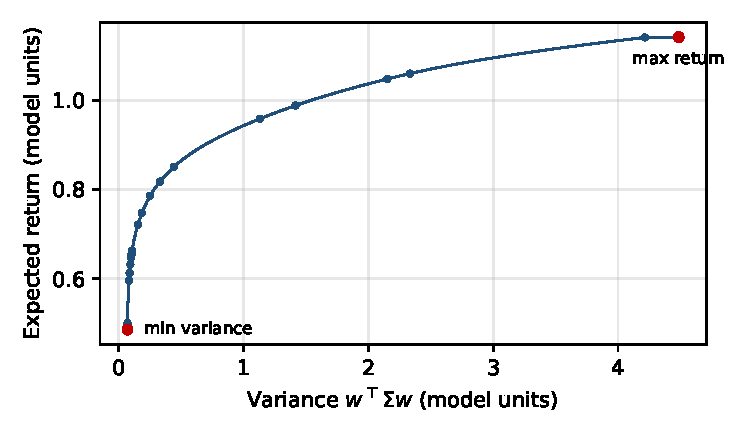
\includegraphics[width=0.65\textwidth]{frontier.pdf}
\caption{The efficient frontier of a $20$-asset long-only problem, traced exactly by
\pkg{cvxcla} as $20$ turning points, plotted as return against variance (\target{frontier}).}
\label{fig:frontier}
\end{center}

The mean--variance portfolio selection problem \citep{markowitz1952} asks for the
allocation of capital across $n$ assets that minimises risk for a given level of
expected return; sweeping the return level produces a one-parameter family of optimal
portfolios whose risk--return image is the \emph{efficient frontier}. The Critical Line
Algorithm (CLA) of \citet{markowitz1956, markowitz1959} represents this frontier
\emph{exactly and in full}: it returns a finite list of \emph{turning points} between
which the frontier is described in closed form, so no discretisation or repeated
re-optimisation is required. The canonical description and a reference implementation
are due to \citet{markowitz2000}; \citet{perold1984}, \citet{stein2008}, and
\citet{hirschberger2010} develop large-scale and active-set variants,
\citet{niedermayer2010} a careful fast implementation, \citet{bailey2013} a widely used
open-source one, and \citet{markowitz2021} a recent review extending the method to
mean--semivariance. In optimisation terms the CLA solves a parametric quadratic
program. \citet{wolfe1959} adapted the simplex method to quadratic programs,
\citet{best1996} gave a parametric active-set algorithm that \citet{best2010} applies to
portfolios, and \pkg{qpOASES} \citep{ferreau2014} is a general parametric QP solver.

Classical CLA implementations take the covariance as a dense matrix. For a large
universe it usually has more structure than that: multi-factor risk models, which
generalise the single-index model \citep{sharpe1963}, write it as a diagonal matrix
plus a low-rank term. The large-scale methods cited above exploit structure through
incremental factorisations, sparsity, or pivoting tied to an explicit matrix.
\pkg{cvxcla} computes the same turning points as any CLA; its contribution is an
\emph{interface} that makes the loop independent of how the covariance is stored, so
the structure becomes a property of an exchangeable backend
(Appendix~\ref{sec:baileydetail}). The mathematics connecting the CLA to the
constrained LASSO, and its history, are the subject of a companion paper
\citep{schmelzer2026perspective}, and \citet{schmelzer2026lasso} shows how to obtain the
efficient frontier from a LASSO solver; this paper documents the software.

\paragraph{Contributions.}
\begin{enumerate}\setlength{\itemsep}{2pt}
\item \textbf{An operator interface.} The turning-point loop reaches the covariance
through a five-member protocol (\S\ref{sec:operators}). A diagonal-plus-low-rank
backend solves the free block through the Woodbury identity, never forms an
$n\times n$ matrix, and traces the same turning points about $40\times$ faster than the dense
backend at $n=2560$, in under $1$~MiB of working memory against $100$~MiB
(\S\ref{sec:experiment}).
\item \textbf{General linear constraints.} Box bounds combine with any linear
equalities $A w = b$ and inequalities $G w \le h$ (\S\ref{sec:ineq}) and a
gross-exposure cap $\lVert w\rVert_1 \le c$ (\S\ref{sec:leverage}).
\item \textbf{A tested implementation.} A least-index tie-break makes the trace
deterministic and provably finite under standard assumptions (\S\ref{sec:bland}); an
independent KKT certificate validates every trace (\S\ref{sec:exactness}); inputs
outside the supported domain are declined with an error that names the cause
(\S\ref{sec:errors}); and one script regenerates every figure and number.
\end{enumerate}
Table~\ref{tab:compare} sets these capabilities against the software a user would
otherwise reach for.

\begin{table}[t]
\centering
\small
\setlength{\tabcolsep}{4pt}
\renewcommand{\arraystretch}{1.5}
\newcolumntype{L}[1]{>{\raggedright\arraybackslash}p{#1}}
\begin{tabular}{L{0.21\textwidth}L{0.20\textwidth}L{0.15\textwidth}L{0.18\textwidth}L{0.13\textwidth}}
\hline
Software & Output & Covariance & Constraints & Gross cap \\
\hline
\pkg{PyPortfolioOpt} \code{CLA} & turning points, some lost & dense matrix & box bounds, one budget row & no \\
QP over a $\lambda$ grid & one portfolio per grid point & as the solver accepts it & any convex & reformulated \\
\pkg{qpOASES} via \pkg{CasADi} & path followed, endpoint returned & matrix & general linear & reformulated \\
\pkg{cvxcla} & every turning point & any operator & box bounds, $Aw=b$, $Gw\le h$ & native lift \\
\hline
\end{tabular}
\caption{What each route to the mean--variance frontier delivers, as used in
\S\ref{sec:experiment}: the QP over a $\lambda$ grid is described in \S\ref{sec:clarabel},
\pkg{qpOASES} in \S\ref{sec:qpoases}, \pkg{cvxcla}'s covariance operators in
\S\ref{sec:operators} and its lift of the gross cap in \S\ref{sec:leverage}. ``Gross
cap'' is $\lVert w\rVert_1 \le c$. ``Path followed, endpoint returned'' means
\pkg{qpOASES} passes the same turning points but does not expose them through
\pkg{CasADi}. The termination
guarantee (\S\ref{sec:bland}) and the KKT certificate (\S\ref{sec:exactness}) are
properties of \pkg{cvxcla}'s trace and are not compared here.}
\label{tab:compare}
\end{table}

We do \emph{not} claim the fastest solve: on small problems \pkg{qpOASES} is faster
(\S\ref{sec:qpoases}), and large dense problems admit faster incremental
factorisations (\S\ref{sec:baseline}).

The package \citep{cvxcla}\footnote{\href{\repourl}{\texttt{github.com/cvxgrp/cvxcla}}}
is built around the class \code{CLA} in \srcfile{src/cvxcla/cla.py}{src/cvxcla/cla.py},
supported by \srcfile{src/cvxcla/first.py}{first.py} (the starting portfolio),
\srcfile{src/cvxcla/operators/__init__.py}{operators/} (the covariance backends), and
\srcfile{src/cvxcla/types.py}{types.py} (the turning-point and frontier data
structures). The notation follows the code.

Sections~\ref{sec:problem}--\ref{sec:iteration} describe the algorithm,
\S\ref{sec:operators} the operator interface, \S\ref{sec:usage} the user interface and
\S\ref{sec:experiment} the experiments; details and the termination proof are in the
appendices.

\section{Problem formulation}
\label{sec:problem}

Let $w\in\R^n$ be the portfolio weights, $\mu\in\R^n$ the expected returns,
$\Sig\in\R^{n\times n}$ the (symmetric, positive semidefinite) covariance,
$A\in\R^{m\times n}$, $b\in\R^m$ the equality constraints, $G\in\R^{p\times n}$,
$h\in\R^p$ the inequality constraints, and $\lb,\ub$ the bounds. The data $\mu$,
$\Sig$, $A$, $b$, $G$, $h$ must be finite. A bound may be infinite, an unbounded box;
the first turning point is then found by the linear program of \S\ref{sec:first}, which
refuses a problem whose expected return is unbounded. The
implementation traces the frontier through the \emph{return-parametrised} quadratic
program
\begin{equation}
\label{eq:qp}
\min_{w\in\R^n}\; \tfrac12\, w\trans \Sig\, w - \lambda\,\mu\trans w
\quad\text{subject to}\quad A w = b,\;\; G w \le h,\;\; \lb \le w \le \ub,
\end{equation}
where $\lambda \ge 0$ weights expected return against variance. The canonical instance
has the single budget row $\mathbf{1}\trans w = 1$; general $A$ and $G$ (group or sector
caps, a $\ge$ row negated) are handled in \S\ref{sec:first} and \S\ref{sec:ineq}. As $\lambda$ decreases from $+\infty$ to $0$, the optimiser moves from the
maximum-return portfolio to the global minimum-variance portfolio, and its locus is the
efficient frontier (Figure~\ref{fig:frontier}).


\paragraph{Optimality conditions.}
At fixed $\lambda$ the program is convex, so the KKT conditions are necessary and
sufficient. Partition the assets into a \emph{free} set $\F$ (weights strictly inside
their bounds) and a \emph{blocked} set $\B = \F^{c}$ (weights at $\lb_i$ or $\ub_i$),
and let $\Sset \subseteq \{1,\dots,p\}$ index the \emph{active} inequality rows. For
the free assets
\begin{equation}
\label{eq:kkt}
\begin{aligned}
\Sig_{\F\F}\, w_\F + \Sig_{\F\B}\, w_\B + A_\F\trans \nu + G_{\Sset\F}\trans \eta
  &= \lambda\, \mu_\F,\\
A_\F\, w_\F + A_\B\, w_\B &= b, \qquad
G_{\Sset\F}\, w_\F + G_{\Sset\B}\, w_\B = h_{\Sset},
\end{aligned}
\end{equation}
with multipliers $\nu\in\R^m$ and $\eta\in\R^{|\Sset|}_{\ge 0}$. The blocked weights
are known, so \eqref{eq:kkt} is linear in $(w_\F,\nu,\eta)$, and an active inequality
row enters exactly as an equality row: stacking $C = [\,A;\,G_{\Sset}\,]$ recovers the
equality-only form.

\paragraph{The affine segment.}
While the partition is fixed, the system matrix is constant and the right-hand side
affine in $\lambda$, so
\begin{equation}
\label{eq:segment}
w(\lambda) = \alpha + \lambda\,\beta,
\end{equation}
with $\alpha,\beta$ constant on the segment ($\beta_\B = 0$, $\alpha_\B = w_\B$); the
code calls them \code{r\_alpha} and \code{r\_beta}. This is the \emph{critical line}.
A \emph{turning point} is a value of $\lambda$ at which the partition must change.

\section{The first turning point}
\label{sec:first}

At $\lambda = +\infty$ variance is irrelevant and \eqref{eq:qp} reduces to earning the
most expected return the constraints allow. For a single all-ones budget row
$\mathbf{1}\trans w = b$, \code{init\_algo}
(\srcfile{src/cvxcla/first.py}{first.py}) computes this greedily: start every weight at
$\lb$, sort the assets by descending $\mu$, and raise each towards $\ub_i$ until the
budget is met (within a tolerance of $10^{-12}$; without it, round-off can skip the
asset that should end strictly inside its box). The last asset touched absorbs the residual and is the
single \emph{free} asset; all others are blocked. The same fill serves leverage
($b > 1$) and dollar-neutral books ($b = 0$, negative $\lb$). The last asset is marked
free even when it lands exactly on a bound, so the reduced KKT system is non-singular
from the outset, a case the review of \citet{markowitz2021} does not address.

For a general equality system (weighted rows, or $m > 1$ rows such as sector or factor
neutrality) or any $G$, the maximum-return vertex is the linear program
$\max_w \mu\trans w$ subject to the constraints, which \pkg{cvxcla} solves with the
HiGHS simplex through \code{scipy.optimize.linprog}; the free set is read off as the
assets strictly inside their bounds. Only this first step differs; the loop that
follows is written for a general $A$ throughout.

\paragraph{Tied maximum returns.}
The maximum-return set need not be a single vertex. When two or more assets share the
largest expected return, say because they were given the same forecast, the linear
program has a whole face of optima, and the greedy fill or the simplex returns one of
its vertices. The frontier does not start at an arbitrary one. For $\lambda$ just below
$+\infty$ the optimiser of \eqref{eq:qp} is the point of that face where the quadratic
term $\tfrac12 w\trans\Sig w$ is smallest, and the path leaves from there. Since
release~2.6.0, \pkg{cvxcla} starts at that point, a small quadratic program over the
face, and its free set is the assets strictly inside their bounds there. Earlier
releases started at the vertex the solver returned. Release~2.3.3, used for the first
version of this paper, then traced a frontier that ended but was not efficient; that
version reported such problems as completed (Appendix~\ref{sec:degeneracy}).
Releases~2.4.2 to 2.5.0 declined them instead.

The vertex itself can be degenerate, with every weight on a bound or a duplicated tight
row. Its partition is then read from a vertex of the linear program's optimal dual set,
which keeps it dual feasible and starts the first segment at the vertex itself
(Appendix~\ref{sec:vertexdetail}). Redundant equality rows, a repeated budget say, are
dropped before the trace starts; a vertex is refused with a \code{DegenerateProblemError}
(\S\ref{sec:errors}) only when its optimal dual set has no vertex.

\section{The turning-point iteration}
\label{sec:iteration}

From the first turning point the algorithm repeatedly (i) solves the reduced KKT system
for the affine segment \eqref{eq:segment}; (ii) finds the largest $\lambda$ below the
current one at which an \emph{event} occurs; (iii) flips the status of the single
coordinate responsible; and (iv) records the new turning point, stopping at
$\lambda = 0$.

\subsection{Solving the reduced KKT system by block elimination}
\label{sec:blockelim}

Write $C_\F$ for the active constraint rows restricted to the free set ($A_\F$ when
$\Sset = \varnothing$; \S\ref{sec:ineq}) and $c$ for their right-hand side. The
reduced system is the saddle-point problem
\begin{equation}
\label{eq:saddle}
\begin{bmatrix} \Sig_{\F\F} & C_\F\trans \\[2pt] C_\F & 0 \end{bmatrix}
\begin{bmatrix} w_\F \\ \nu \end{bmatrix}
=
\begin{bmatrix} r_1 \\ r_2 \end{bmatrix},
\end{equation}
solved for two right-hand sides at once, the ``$\alpha$ system''
$r_1^{\alpha} = -\Sig_{\F\B} w_\B$, $r_2^{\alpha} = c - C_\B w_\B$, and the
``$\beta$ system'' $r_1^{\beta} = \mu_\F$, $r_2^{\beta} = 0$. Rather than factor the
full saddle matrix, the code eliminates the free block. A single multi-column solve
against $\Sig_{\F\F}$ gives $Y = \Sig_{\F\F}\inv C_\F\trans$ and
$z^{\alpha,\beta} = \Sig_{\F\F}\inv r_1^{\alpha,\beta}$. The multipliers come from the
small Schur complement $S = C_\F Y$. With $n_\F$ free assets and $m_c = m + |\Sset|$ active rows,
$C_\F \in \R^{m_c\times n_\F}$, $Y \in \R^{n_\F\times m_c}$ and $S \in \R^{m_c\times m_c}$,
\begin{equation}
\label{eq:schur}
\nu^{\alpha} = S\inv\!\left(C_\F z^{\alpha} - r_2^{\alpha}\right),
\qquad
\nu^{\beta} = S\inv C_\F z^{\beta},
\end{equation}
and back-substitution gives
\begin{equation}
\label{eq:freesoln}
\alpha_\F = z^{\alpha} - Y\nu^{\alpha},
\qquad
\beta_\F = z^{\beta} - Y\nu^{\beta}.
\end{equation}
The dominant cost is the solve against $\Sig_{\F\F}$; for the plain budget $S$ is a
scalar. With $1 < m_c \le n_\F$ the rows are first replaced by an orthonormal basis of
their span, $C_\F\trans = QR$, and the system is solved with $Q$ in place of
$C_\F\trans$, the target $R^{-\mathsf{T}} r_2$, and the multipliers recovered by a
triangular solve with $R$. The condition number of $C_\F \Sig_{\F\F}\inv C_\F\trans$ can
reach $\operatorname{cond}(\Sig_{\F\F})\operatorname{cond}(C_\F)^2$, while
$Q\trans\Sig_{\F\F}\inv Q$ is no worse conditioned than $\Sig_{\F\F}$, so nearly
dependent active rows lose accuracy in proportion to $\operatorname{cond}(C_\F)$, the
sensitivity of the constraint data, and not to its square. Solving only for the free block keeps every step a dense solve of size
$|\F|$, where \citet{markowitz2021} assemble one large KKT system over all variables.

To decide when a blocked asset should re-enter, the code forms the reduced gradients
\begin{equation}
\label{eq:gamma}
\gamma = \Sig\,\alpha + C\trans \nu^{\alpha}, \qquad
\delta = \Sig\,\beta + C\trans \nu^{\beta} - \mu,
\end{equation}
where $\nu$ stacks the equality and active-row multipliers, so that $\gamma_i + \lambda\delta_i$ is (proportional to) the bound multiplier of a
blocked asset $i$ along the segment; the products $\Sig\alpha$, $\Sig\beta$ go through
the covariance operator of \S\ref{sec:operators}.

\subsection{Event detection}
\label{sec:events}

The segment stays optimal until one of four events changes the active set. Two act on
variables through the box bounds:
\begin{itemize}
\item \textbf{Free $\to$ blocked.} A free weight $w_i = \alpha_i + \lambda\beta_i$ meets
its upper bound at $\lambda_i = (\ub_i - \alpha_i)/\beta_i$ when $\beta_i < 0$, or its
lower bound at $\lambda_i = (\lb_i - \alpha_i)/\beta_i$ when $\beta_i > 0$.
\item \textbf{Blocked $\to$ free.} A blocked asset's multiplier changes sign at
$\lambda_i = -\gamma_i/\delta_i$, admissible at the upper bound with $\delta_i < 0$ or
the lower bound with $\delta_i > 0$.
\end{itemize}
The other two are the same moves on the rows of $G w \le h$, described in
\S\ref{sec:ineq}. The candidates form a matrix $L\in\R^{(n+p)\times 4}$, one row per
variable or inequality row, with $-\infty$ where an event cannot occur, under two
numerical guards:
\begin{itemize}
\item \textbf{Slope floor.} A slope at round-off level is treated as zero. The floor is
$\sqrt{\varepsilon_{\text{mach}}}$ in the problem's own units, so the trace is
invariant to rescaling $\mu$ or $\Sig$ (Appendix~\ref{sec:guards}).
\item \textbf{$\lambda$ window.} Candidates above the current $\lambda$, beyond a
relative $10^{-10}$, lie outside the segment and are discarded; the same window decides
which events are tied.
\end{itemize}
The next turning point is $\lambda^{\star} = \max_{i,t} L_{it}$; if
$\lambda^{\star} \le 0$ the frontier is complete.

\subsection{General linear inequalities}
\label{sec:ineq}

A row of $G w \le h$ is the analogue of a box bound: either \emph{active}
($g_j\trans w = h_j$) or slack. While active it is carried through the reduced solve as
an extra equality row, stacked under $A$ into $C_\F = [\,A_\F;\,G_{\Sset\F}\,]$, so each
step is still one solve against $\Sig_{\F\F}$ (through the operator interface) feeding
an $(m+|\Sset|)$-dimensional Schur complement. The box bounds stay a separate per-variable
active set, so the box-only problem pays nothing for the generalisation.

The stacked solve \eqref{eq:schur} returns an affine multiplier
$\eta_j(\lambda) = \eta_j^{\alpha} + \lambda\,\eta_j^{\beta}$ for each active row, and
the two row events mirror the box events:
\begin{itemize}
\item \textbf{Activate.} An inactive row with slack
$s_j(\lambda) = (g_j\trans\alpha - h_j) + \lambda\,g_j\trans\beta$ binds at
$\lambda_j = (h_j - g_j\trans\alpha)/(g_j\trans\beta)$, admissible when
$g_j\trans\beta < 0$ (the slack rises as $\lambda$ falls).
\item \textbf{Release.} An active row releases at
$\lambda_j = -\eta_j^{\alpha}/\eta_j^{\beta}$, where its multiplier reaches zero,
admissible when $\eta_j^{\beta} > 0$.
\end{itemize}
These fill the trailing $p$ rows of $L$, so a group cap or factor-exposure band is
traced along the whole frontier (\S\ref{sec:exactness}). Each active row adds a column
to the solve against $\Sig_{\F\F}$ and a row to the Schur complement; with many active
rows that term, not the covariance solve, dominates a step. A row that is tight but a combination of the active rows on the
free set is supported: at the first vertex only an independent subset of the tight rows
is made active (\S\ref{sec:first}), and during the trace such a row has zero slope,
$g_j\trans\beta = 0$ (since $C_\F\beta_\F = 0$), so its activation event does not fire.
The active rows themselves must stay linearly independent on the free set, or the Schur
complement is singular, as when several caps bind at once in the same direction. Before
each solve the rows are tested, and a dependent set is refused with a
\code{DegenerateProblemError} at that $\lambda$.

\subsection{Gross-exposure caps}
\label{sec:leverage}

A cap $\lVert w\rVert_1 \le c$ on gross exposure (under a full budget, $c = 1.3$ is a
130/30 book) is polyhedral but not a single row of $G$. The code lifts it. Each asset
whose box straddles zero is split into a long and a short leg, $w_i = x_i^+ - x_i^-$
with $x_i^+\in[0,\ub_i]$ and $x_i^-\in[0,-\lb_i]$; a long-only or short-only asset keeps one
leg, so a long-only problem is not enlarged. With $w = Px$ for the signed
leg-to-asset map, the cap becomes the one row $\mathbf{1}\trans x \le c$ appended to
$GP$, the other constraints carry over as $AP$ and $GP$, and the mean becomes
$P\trans\mu$. The lifted program is an instance of \eqref{eq:qp} with the same
$\lambda$, traced by the loop above and mapped back through $P$ (validated in
\S\ref{sec:exactness}).

The lifted covariance $P\trans\Sig P$ is singular, since raising both legs of one
asset leaves $w$ unchanged. The loop never meets that singularity: both legs of an asset
are never free together, so every free block is a signed principal submatrix of $\Sig$,
served through the operator interface without forming $P\trans\Sig P$, and a factor
backend keeps its Woodbury solve. Appendix~\ref{sec:liftdetail} gives the argument and
two edge cases of the first vertex.

\subsection{Anti-cycling and termination}
\label{sec:bland}

On degenerate problems (tied returns, exchangeable assets, several constraints active at
once) several events can share $\lambda^{\star}$, and a naive rule can cycle. Among all
events within tolerance of $\lambda^{\star}$ the implementation picks the lowest
coordinate index, and within it the lowest event column, and flips that coordinate
alone. Call a partition (free set, blocked bounds, active rows $\Sset$) \emph{valid} at
$\lambda$ when its segment respects the bounds and the inactive rows there and its
multipliers have the right signs.

\begin{proposition}\label{prop:termination}
Let $\Sig \succ 0$, and suppose that at every turning point the constraints holding
with equality (the rows of $A$, the rows of $G$ with $g_j\trans w = h_j$, and the
bounds on which a weight sits) have linearly independent gradients. Then, in exact
arithmetic, the walk never returns to a partition it has left, and it reaches
$\lambda = 0$ after finitely many turning points.
\end{proposition}

\begin{proof}[Outline]
A partition stays valid while finitely many conditions, each affine in $\lambda$,
hold; once one fails below a turning point it fails for every smaller $\lambda$, so a
partition never recurs at a later $\lambda$, and without ties every step uses a new one.
At a tie, the slope of the next segment solves a strictly convex QP whose KKT system is a
linear complementarity problem with a positive-definite matrix, and the implementation's
lowest-index single flip is Murty's least-index principal pivot on it, which is finite.
Appendix~\ref{sec:proof} gives the full argument, including the correspondence between
the event types of the code and the complementary pairs of the problem.
\end{proof}

The proposition holds in exact arithmetic and under its hypotheses; what it adds is that
the walk never revisits a partition. Two weaker statements hold without them. Because
$\Sig \succ 0$ the optimiser $w(\lambda)$ is unique, and for a fixed set of active
constraints it is affine in $\lambda$ on the interval where that set is optimal; there
are finitely many such sets, so the frontier itself has finitely many turning points
whether or not the constraints are independent. And an iteration cap of $100(n+p+1)$
stops every trace: a trace that reaches it raises an error and never returns a partial
frontier, and no trace in Appendix~\ref{sec:degeneracy} used more than $1.5\%$ of it.
In exact arithmetic, then, the one thing left unproved outside the hypotheses is that
the walk leaves every tie without revisiting a partition. This concerns a degenerate maximum-return vertex,
resolved from a vertex of its optimal dual set, or, under tied maximum returns, from the
minimiser of the quadratic term on the tied face (\S\ref{sec:first}); a singular $\Sig$
that the active rows keep positive definite on their null space, outside
$\Sig\succ0$ (Appendix~\ref{sec:degeneracy}); the lifted problem
of \S\ref{sec:leverage}, whose singular covariance masks the competing leg events; and
ties with dependent constraints, where the matrix $M$ of Appendix~\ref{sec:proof} is
only positive semidefinite and the least-index result no longer applies (a partition
with dependent active rows is refused, \S\ref{sec:ineq}). Appendix~\ref{sec:degeneracy}
lists which test families satisfy the hypotheses. In floating point the tie window and
the slope floor make the computed signs agree with the exact ones, which is not proved
either. At run time every turning point is validated against the bounds, $A w = b$ and
$G w \le h$ before it is accepted, and the KKT certificate of \S\ref{sec:exactness}
checks the traces of \S\ref{sec:experiment} and Appendix~\ref{sec:degeneracy} for
optimality.

When no admissible event has a positive ratio the walk has reached the minimum-variance
portfolio and appends a final turning point $w = \alpha$ at $\lambda = 0$.

\begin{center}
\fbox{\begin{minipage}{0.93\textwidth}
\textbf{Algorithm 1.}~Critical Line Algorithm (as implemented in \pkg{cvxcla}).

\smallskip
\textit{Input:} $\mu$, $\Sig$, $\lb,\ub$, $A,b$, $G,h$, tolerance $\tau$.
\begin{enumerate}\setlength{\itemsep}{1pt}
\item Compute the maximum-return vertex (\S\ref{sec:first}); record its free set and
      active rows $\Sset$ with $\lambda \gets \infty$.
\item \textbf{While} $\lambda > 0$:
  \begin{enumerate}\setlength{\itemsep}{1pt}
  \item Fix $w_\B$ at the active bounds and stack $C_\F = [\,A_\F;\,G_{\Sset\F}\,]$.
  \item Solve against $\Sig_{\F\F}$ for $Y$, $z^{\alpha}$, $z^{\beta}$; solve the Schur
        system \eqref{eq:schur}; back-substitute \eqref{eq:freesoln} for
        $\alpha,\beta$; form $\gamma,\delta$ \eqref{eq:gamma}.
  \item Assemble $L$ (\S\ref{sec:events}, \S\ref{sec:ineq}) under the slope floor and
        $\lambda$ window; $\lambda^{\star} \gets \max L$; \textbf{if}
        $\lambda^{\star} \le 0$ \textbf{break}.
  \item Pick the event by the least-index rule (\S\ref{sec:bland}), flip that
        coordinate's status, set
        $\lambda \gets \lambda^{\star}$, append $w = \alpha + \lambda^{\star}\beta$.
  \end{enumerate}
\item Append $w = \alpha$ at $\lambda = 0$ and \textbf{return} the turning points.
\end{enumerate}
\end{minipage}}
\end{center}

\section{The covariance operator abstraction}
\label{sec:operators}

The design separates the path-following algorithm from the storage and solution of the
quadratic form (Figure~\ref{fig:design}). The turning-point loop needs only three
operations on the covariance: a matrix--vector product $\Sig x$, a multi-column solve
against the free block $\Sig_{\F\F}\inv R$, and the free-to-blocked cross product
$\Sig_{\F\B}\,x_\B$, which is formed from the first. A backend supplies them through the
protocol \code{QuadraticForm} (alias \code{CovarianceOperator}, the
\code{SymmetricOperator} contract of \pkg{cvx-linalg}), whose five members are listed in
Table~\ref{tab:protocol}; two of them serve the gross-exposure lift and the singularity
guard. The algorithm never assumes an explicit matrix, and it assumes of a backend only
that $\Sig$ is symmetric and that every free block it solves is positive definite on
the null space of the active rows, which \code{rcond\_free} lets it check before
trusting the solve (Appendix~\ref{sec:degeneracy}). Four backends ship with the package, and a user can add
others without touching the loop (\S\ref{sec:custom}).

\begin{figure}[t]
\centering
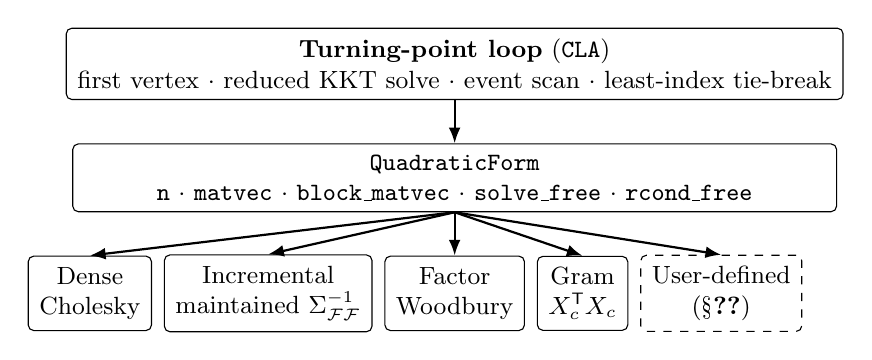
\begin{tikzpicture}[
  box/.style={draw, rounded corners=2pt, align=center, font=\small, inner sep=4pt},
  arrow/.style={-{Latex[length=2mm]}, thick}]
\node[box, minimum width=0.8\textwidth] (loop) {\textbf{Turning-point loop} (\code{CLA})\\
  first vertex $\cdot$ reduced KKT solve $\cdot$ event scan $\cdot$ least-index tie-break};
\node[box, below=0.55cm of loop, minimum width=0.8\textwidth] (proto) {\textbf{\code{QuadraticForm}}\\
  \code{n} $\cdot$ \code{matvec} $\cdot$ \code{block\_matvec} $\cdot$ \code{solve\_free} $\cdot$ \code{rcond\_free}};
\node[box, below=0.55cm of proto] (fac) {Factor\\Woodbury};
\node[box, left=0.15cm of fac] (inc) {Incremental\\maintained $\Sig_{\F\F}\inv$};
\node[box, left=0.15cm of inc] (dense) {Dense\\Cholesky};
\node[box, right=0.15cm of fac] (gram) {Gram\\$X_c\trans X_c$};
\node[box, right=0.15cm of gram, dashed] (user) {User-defined\\(\S\ref{sec:custom})};
\draw[arrow] (loop) -- (proto);
\foreach \b in {dense, inc, fac, gram, user} \draw[arrow] (proto.south) -- (\b.north);
\end{tikzpicture}
\caption{The covariance enters the turning-point loop only through the
\code{QuadraticForm} protocol; the backends below it are interchangeable.}
\label{fig:design}
\end{figure}

\begin{table}[t]
\centering
\small
\begin{tabular}{p{0.32\textwidth}p{0.29\textwidth}p{0.28\textwidth}}
\hline
Member & Returns & Used for \\
\hline
\code{n} & the number of assets & sizes \\
\code{matvec(x)} & $\Sig x$, for a vector or a matrix $x$ & gradients, the cross product \\
\code{block\_matvec(rows, cols, v)} & $\Sig_{\text{rows},\text{cols}}\, v$ & the gross-exposure lift (\S\ref{sec:leverage}) \\
\code{solve\_free(free, R)} & $\Sig_{\F\F}\inv R$ & the reduced KKT solve (\S\ref{sec:blockelim}) \\
\code{rcond\_free(free)} & the reciprocal condition number of $\Sig_{\F\F}$ & the singularity guard \\
\hline
\end{tabular}
\caption{The \code{QuadraticForm} protocol. Index sets are integer arrays into $\{0,\dots,n-1\}$.}
\label{tab:protocol}
\end{table}

\paragraph{Dense.} \code{DenseCovariance} wraps an explicit matrix and solves the free
block by Cholesky (\code{scipy.linalg.cho\_factor}), falling back to LU on the rare
block that is not numerically positive definite. It reproduces the classical CLA and is
the reference backend.

\paragraph{Incremental dense.}
\label{sec:incremental}
\code{IncrementalDenseCovariance} traces the same turning points but \emph{maintains}
$\Sig_{\F\F}\inv$: because the free set changes by one asset per turning point, a
bordered rank-one update or a symmetric deletion costs $O(n_\F^2)$ against a fresh
$O(n_\F^3)$ factorisation, which makes a trace about twice as fast at $n=320$, three times at $n=640$, and seven times at $n=2560$ (\S\ref{sec:baseline}). A non-positive Schur pivot or a multi-asset change triggers a full refactorisation. The
backend passes the same KKT certificate as the dense one (Table~\ref{tab:kkt}), but a
maintained inverse carries round-off from step to step over the roughly $n$ updates of
a trace, so it is opt-in.

\paragraph{Factor (diagonal-plus-low-rank).}
\code{FactorCovariance} represents
\begin{equation}
\label{eq:factor}
\Sig = \operatorname{diag}(d) + U\,\Delta\,U\trans,
\qquad d\in\R^{n}_{>0},\; U\in\R^{n\times K},\; \Delta\in\R^{K\times K},
\end{equation}
the form of factor models \citep{sharpe1963} and of eigenvalue-clipped covariances. The
free-block solve never forms $\Sig_{\F\F}$; it uses the Woodbury identity
\begin{equation}
\label{eq:woodbury}
\Sig_{\F\F}\inv = D_\F\inv - D_\F\inv U_\F\, W\inv\, U_\F\trans D_\F\inv,
\qquad
W = \Delta\inv + U_\F\trans D_\F\inv U_\F \in\R^{K\times K},
\end{equation}
so a solve costs $O(n_\F K^2 + K^3)$ rather than $O(n_\F^3)$, storage is $O(nK)$, and
the cross product is $U_\F\,\Delta\,(U_\B\trans x_\B)$. The same free-block algebra serves a
single constrained solve as well: \citet{schmelzer2026nncg} reach the free block of a
non-negative QP through the same Woodbury inverse and factored products.

The admissible model is $d > 0$ and $\Delta$ symmetric positive semidefinite.
\code{FactorCovariance} folds $\Delta$ into the loadings when it is built: with
$\Delta = V\Lambda V\trans$ it stores $U' = U V_+ \Lambda_+^{1/2}$, the directions of
positive variance, and an identity inner matrix, which is the same $\Sig$. The
Woodbury solve \eqref{eq:woodbury} then runs with $U'$ and $W = I + U_\F'^{\mathsf{T}}
D_\F\inv U_\F'$ and never inverts $\Delta$. A singular factor covariance, from a factor
with zero variance or perfectly correlated factors, is therefore admissible, and its rank
$K$ is the number of directions kept. An indefinite $\Delta$ is refused: a signed
low-rank term can still give a positive-definite $\Sig$, but $W$ would then be
indefinite, so such a covariance is passed as a dense matrix. Since $d > 0$, $W$ is
positive definite, and the factor solve needs no guard of its own beyond the one on
$\Sig_{\F\F}$. Against the dense trace of the same $\Sig$, the factor trace has the same
turning points and weights equal to $2.8\times10^{-12}$, with KKT residuals below
$2.3\times10^{-13}$, for $\Delta$ with condition numbers up to $10^{14}$, loadings
collinear to within $10^{-10}$, and the full rank $K = n = 120$
(\target{validate-factor}). Every active constraint row adds a column to the solve and a
row to the Schur complement, so with many active rows that term dominates the cost. A low-rank \emph{approximation} of a sample covariance traces the frontier of
the approximation, which is a different frontier (\S\ref{sec:estimators}).

\paragraph{Data matrix (Gram).}
\label{sec:gram}
A sample covariance is a Gram matrix: for the column-centred returns
$X_c\in\R^{T\times n}$, $\Sig = X_c\trans X_c/(T-1)$. \code{GramCovariance} implements
the protocol straight from $X_c$ in $O(Tn)$ storage. When $T<n$ the matrix is singular,
and once the free set outgrows the data rank the free block is singular too; the active
rows still hold it on their null space, where it is solved (Appendix~\ref{sec:degeneracy}).
An optional ridge $\theta I$ (the argument \code{ridge}) makes $\Sig$ positive definite,
a different, regularised frontier, and the solve is then Woodbury in the
$T$-dimensional observation space. The saving is in storage: when the dense matrix fits,
\code{DenseCovariance} is faster per step, and the structured route pays only while $T$
(or $K$) stays well below $n$ (\S\ref{sec:rankscaling}).

\subsection{Regularization through the operator}
\label{sec:regularization}

A quadratic penalty $\tfrac{\theta}{2}\, w\trans M w$, with $\theta \ge 0$ and $M$
symmetric positive semidefinite and independent of $\lambda$, changes only the Hessian,
so the path stays piecewise linear and the penalty is the substitution
$\Sig \mapsto \Sig + \theta M$: a ridge ($M = I$) or a factor-exposure penalty
($M = B B\trans$ for exposures $B$). \code{CLA} has no penalty argument; the regularized
form is supplied as the covariance, a bundled or a user-written \code{QuadraticForm}
(\S\ref{sec:custom}). \code{GramCovariance} with $\theta>0$ and \code{FactorCovariance}
already are such forms. A rank-deficient sample covariance needs neither: its frontier
is traced as it is, as long as the active rows keep the free block positive definite on
their null space (Appendix~\ref{sec:degeneracy}). A small ridge or a factor model is the
fix when they do not, and a choice of estimator otherwise (\S\ref{sec:estimators}). A penalty centred on a nonzero portfolio $w_0$ (tracking
error, quadratic turnover) adds the linear term $-\theta\, w\trans M w_0$, which the
interface does not expose; nonquadratic penalties such as linear transaction costs lie
outside the method.

\subsection{Writing a backend}
\label{sec:custom}

A backend is a subclass of \code{QuadraticForm} that implements the five members of
Table~\ref{tab:protocol}. For a block-diagonal covariance, assets in groups with no
cross-group covariance (a structure the package does not ship), the free-block solve
splits into one Cholesky solve per block. The two members that carry the structure are
below; \code{n}, \code{matvec} and \code{block\_matvec} are a few lines each, and the
complete, runnable class is in the package documentation
(\srcfile{docs/custom-backend.md}{docs/custom-backend.md}).

\begin{CodeInput}
class BlockDiagonal(QuadraticForm):   # Sigma = blockdiag(S_1, ..., S_m)
    def solve_free(self, free, rhs):
        out = np.empty_like(rhs, dtype=float)
        # one (positions, free sub-block) pair per group
        for pos, sub in self._parts(free):
            out[pos] = cho_solve(cho_factor(sub), rhs[pos])
        return out

    def rcond_free(self, free):
        eig = np.concatenate(
            [np.linalg.eigvalsh(sub) for _, sub in self._parts(free)]
        )
        return eig.min() / eig.max()
\end{CodeInput}

\code{CLA} runs on it unchanged: on four groups of five assets it traces the same $19$
turning points as the dense matrix. The package's test suite,
\srcfile{tests/test_custom_backend.py}{tests/test\_custom\_backend.py}, checks the same
with general constraints and with a gross-exposure cap, which goes through
\code{block\_matvec}.
The frontier is exact to the accuracy of \code{solve\_free}; an approximate solver
traces the frontier of the matrix it effectively applies, and the KKT certificate of
\S\ref{sec:exactness} checks the result. A sparse matrix
with a sparse Cholesky factor, a Kronecker product, or a matrix-free operator with an
iterative \code{solve\_free} fit the same five members.

\section{Using the package}
\label{sec:usage}

The package \citep{cvxcla} is installed with \code{pip install cvxcla}; it is pure
\proglang{Python} and needs \pkg{NumPy}, \pkg{SciPy} and \pkg{cvx-linalg}
(Computational details). The workflow goes through a single class, \code{CLA}. The user supplies $\mu$, the
covariance (a dense array or any backend of \S\ref{sec:operators}), the bounds, and
the constraints; constructing the object traces the whole frontier. The example traces
a small long-only, fully-invested problem and reads off the maximum-Sharpe portfolio.

\begin{CodeInput}
import numpy as np
from cvxcla import CLA, FactorCovariance

rng = np.random.default_rng(1)
n, k = 6, 2
d = rng.uniform(0.1, 0.5, n)            # idiosyncratic variances
U = rng.standard_normal((n, k))         # factor loadings
Delta = np.diag(rng.uniform(0.5, 2.0, k))
Sigma = np.diag(d) + U @ Delta @ U.T    # a dense 2-factor covariance
mean = rng.standard_normal(n)

cla = CLA(
    mean=mean, covariance=Sigma,
    lower_bounds=np.zeros(n), upper_bounds=np.ones(n),
    a=np.ones((1, n)), b=np.ones(1),    # fully invested: sum(w) = 1
)
print("turning points:", len(cla.turning_points))
sr, w = cla.frontier.max_sharpe
print("max Sharpe:", round(sr, 4))
print("weights:", np.round(w, 3))
\end{CodeInput}

\begin{CodeOutput}
turning points: 7
max Sharpe: 2.4037
weights: [0.    0.    0.704 0.296 0.    0.   ]
\end{CodeOutput}

Switching to a structured backend changes only the covariance argument; because the
factor backend represents the \emph{same} $\Sig$, it returns the same frontier to round-off.

\begin{CodeInput}
factor = FactorCovariance(d=d, u=U, delta=np.diag(Delta))
cla_factor = CLA(
    mean=mean, covariance=factor,
    lower_bounds=np.zeros(n), upper_bounds=np.ones(n),
    a=np.ones((1, n)), b=np.ones(1),
)
w_dense = np.array([t.weights for t in cla.turning_points])
w_factor = np.array([t.weights for t in cla_factor.turning_points])
print("identical frontier:", np.allclose(w_dense, w_factor))
\end{CodeInput}

\begin{CodeOutput}
identical frontier: True
\end{CodeOutput}

A fluent builder, \code{CLA.problem}, assembles the same arguments step by step through
methods such as \code{.budget}, \code{.equality} and \code{.inequality}; an extra \code{.equality} row,
such as a fixed sector weight, makes the first turning point the linear program of
\S\ref{sec:first}.


\subsection{The interface}
\label{sec:api}

\code{CLA} takes the problem as keyword arguments, all \pkg{NumPy} arrays of floats, and
traces the frontier in its constructor. Required are \code{mean} ($\mu$, length $n$),
\code{covariance} (an $n\times n$ array, which is wrapped as a \code{DenseCovariance},
or any backend of \S\ref{sec:operators}), \code{lower\_bounds} and \code{upper\_bounds}
(length $n$), and \code{a}, \code{b} ($m\times n$ and length $m$; a budget is
\code{a = np.ones((1, n))}, \code{b = np.ones(1)}). Optional are \code{g}, \code{h}
($p\times n$ and length $p$) for $Gw \le h$, \code{leverage} for the cap
$\lVert w\rVert_1 \le c$, and \code{tol} (default $10^{-5}$), the tolerance for deciding
that a weight sits on a bound and for validating each turning point; the event ordering
uses its own relative window of at most $10^{-10}$ (\S\ref{sec:events}). The arrays (and a
dense covariance) are copied into read-only arrays when the object is built, so
changing the caller's arrays afterwards cannot put the stored turning points out of step
with the data; a backend is used as given. Non-finite data are refused at this point,
as are NaN bounds. Redundant equality rows are
dropped, and \code{cla.a}, \code{cla.b} then hold the reduced system.

The result is \code{cla.turning\_points}, a list of \code{TurningPoint} objects with the
\code{weights}, the value \code{lamb} of $\lambda$, the boolean mask \code{free} of free
assets, and the mask \code{active\_ineq} of active rows of $G$. The maximum-return
vertex appears twice, at $\lambda = \infty$ and again at the first finite turning point,
where the path leaves it; \code{len(cla)} is the number of turning points.
\code{cla.frontier} wraps them as a \code{Frontier}
(\srcfile{src/cvxcla/types.py}{types.py}), which exposes the \code{weights},
\code{returns}, \code{variance}, \code{volatility} and \code{sharpe\_ratio} of the
turning points and a \code{plot} method. Because the frontier is piecewise linear in
weight space, \code{interpolate(num)} returns intermediate portfolios with no
discretisation error.

\subsection{The frontier and the maximum-Sharpe portfolio}
\label{sec:frontier}

\code{max\_sharpe} maximises $\mu\trans w/\sqrt{w\trans\Sig w}$, the Sharpe ratio with a
zero risk-free rate (supply excess returns as $\mu$ otherwise), over the computed
frontier. On a segment $w(t) = (1-t)\,w_0 + t\,w_1$, $t \in [0,1]$, the return is affine
and the variance quadratic in $t$,
\begin{equation}
S(t) = \frac{a_0 + a_1 t}{\sqrt{c_0 + c_1 t + c_2 t^2}}, \qquad
\begin{aligned}
a_0 &= \mu\trans w_0, & c_0 &= w_0\trans\Sig w_0, & c_2 &= \Delta\trans\Sig\Delta,\\
a_1 &= \mu\trans\Delta, & c_1 &= 2\,w_0\trans\Sig\Delta, & \Delta &= w_1 - w_0,
\end{aligned}
\end{equation}
and the numerator of $S'(t)$ is affine in $t$ (its $t^2$ terms cancel), so $S$ has at
most one stationary point,
\begin{equation}\label{eq:tstar}
t^\star = \frac{a_0 c_1 - 2 a_1 c_0}{a_1 c_1 - 2 a_0 c_2}.
\end{equation}
The maximum on the segment is the largest of $S(0)$, $S(1)$ and, when
$0 < t^\star < 1$, $S(t^\star)$; a stationary point outside the segment is ignored, an
optimum at a turning point is found as an end point, and when $a_1 c_1 = 2 a_0 c_2$ there
is no stationary point and only the end points are compared. The code applies this
rule to every segment of the frontier and returns the best candidate, so the result is
the exact maximum over the computed frontier, without relying on the ratio being
unimodal, at the cost of one matrix--vector product with $\Sig$ per segment.

Points of zero variance are skipped (\code{sharpe\_ratio} reports NaN there); with no
positive variance \code{max\_sharpe} raises a \code{ValueError}, and with no positive
expected return it warns and returns the least negative ratio. Whether the ratio,
computed from estimated $\mu$ and $\Sig$, predicts future performance is a statistical
question outside the package (\S\ref{sec:estimators}).

\subsection{Supported inputs and errors}
\label{sec:errors}




Table~\ref{tab:errors} sorts the inputs into kinds, each with its own exception and
remedy, and each row is a test in the package
(\srcfile{tests/test_errors.py}{tests/test\_errors.py} and
\srcfile{tests/test_degenerate_vertex.py}{tests/test\_degenerate\_vertex.py}). All are raised by the constructor. The package errors derive from \code{CLAError} and also from the built-in
exception raised before (\code{ValueError}, or \code{RuntimeError}), so existing
handlers keep working.



A sample covariance from fewer observations than assets is a case that used to be
declined and no longer is. It is singular, and its free block becomes singular partway
along the frontier. The budget row still holds the free assets on its null space, where
the block stays positive definite, so the trace goes on there (Appendix~\ref{sec:degeneracy}).
A ridged Gram backend (\S\ref{sec:gram}) traces a different, regularised frontier:

\noindent\begin{minipage}{\textwidth}
\begin{CodeInput}
from cvxcla import GramCovariance

returns = 0.01 * rng.standard_normal((4, n)) + 0.001    # 4 days, 6 assets: rank 3
long_only = dict(lower_bounds=np.zeros(n), upper_bounds=np.ones(n),
                 a=np.ones((1, n)), b=np.ones(1))
cla = CLA(mean=returns.mean(axis=0),
          covariance=np.cov(returns, rowvar=False), **long_only)
ridged = CLA(mean=returns.mean(axis=0),
             covariance=GramCovariance(returns, ridge=1e-4), **long_only)
print("turning points:", len(cla), "| with a ridge:", len(ridged))
\end{CodeInput}
\begin{CodeOutput}
turning points: 5 | with a ridge: 7
\end{CodeOutput}
\end{minipage}

Release~2.3.3 declined the first of these. Every turning point of the trace above
matches an interior-point solve of the same quadratic program.

\begin{table}[tb]
\centering
\small
\renewcommand{\arraystretch}{1.25}
\newcolumntype{L}[1]{>{\raggedright\arraybackslash}p{#1}}
\begin{tabular}{@{}L{0.62\textwidth}L{0.32\textwidth}@{}}
\toprule
Input & Remedy \\
\midrule
\multicolumn{2}{@{}l}{\textbf{Malformed input}: \code{ValueError}, before the walk} \\
Non-symmetric $\Sig$; non-finite data or NaN bounds; an indefinite factor $\Delta$;
wrong shapes & correct the data \\
\midrule
\multicolumn{2}{@{}l}{\textbf{Infeasible}: \code{InfeasibleProblemError}, before the walk} \\
Crossed bounds; an unreachable budget; constraints with no feasible point; dependent
equality rows that contradict the others & change the constraints \\
\midrule
\multicolumn{2}{@{}l}{\textbf{Harmless degeneracy}: traced, nothing raised} \\
Redundant equality rows; duplicated, never-binding or locally redundant inequality
rows; a degenerate maximum-return vertex whose optimal dual set has a vertex, and tied
maximum returns (\S\ref{sec:first}); a singular covariance whose free blocks the active
rows keep positive definite (Appendix~\ref{sec:degeneracy}) & -- \\
\midrule
\multicolumn{2}{@{}l}{\textbf{Unsupported degeneracy}: \code{DegenerateProblemError}} \\
Before the walk: a degenerate vertex whose optimal dual set has no vertex, as when a
tight row touches only assets fixed at both bounds; infinite bounds that make the
return unbounded & perturb the bounds or constraints \\
During the walk: a free block singular even on the null space of the active rows, or
active rows dependent on the free set & a ridge or factor model; loosen a cap \\
\midrule
\multicolumn{2}{@{}l}{\textbf{Numerical failure}: \code{NumericalError}, during the walk} \\
Iteration cap; projection fails; a turning point violates a constraint
& regularise $\Sig$ or relax \code{tol}; report it \\
\bottomrule
\end{tabular}
\caption{Supported and unsupported inputs, grouped by the exception each raises and
when, with the usual remedy. ``Before the walk'' is input validation and the first
vertex; ``during the walk'' is a turning point of the trace.}
\label{tab:errors}
\end{table}


\section{Numerical experiment}
\label{sec:experiment}

The experiments answer three questions, in this order: whether the trace is correct
(\S\ref{sec:exactness}); whether its speed on large problems comes from the structured
solve rather than from bookkeeping (\S\ref{sec:scaling}--\S\ref{sec:rankscaling}); and
how it compares with the alternatives, a QP swept over a grid and a parametric QP solver
(\S\ref{sec:clarabel}, \S\ref{sec:qpoases}). A real S\&P 500 frontier closes the section
(\S\ref{sec:empirical}); further checks are in Appendices~\ref{sec:details} and~\ref{sec:degeneracy}. Timings are
the median of three repetitions (bands span their range), each method and size in a
freshly spawned interpreter, on the machine of Computational details. Two complete runs
of the scaling sweep agree to within $10\%$ (median $3\%$) for traces of $10$~ms or more
and to within $40\%$ below that, so ratios are rounded accordingly and those at small
$n$ are indicative only.

\subsection{Correctness: a reference solver and a KKT certificate}
\label{sec:exactness}

On $40$ real assets (\S\ref{sec:empirical}; condition number $\approx 200$) the CLA
traces $29$ turning points. At the midpoint $\lambda$ of each of the $27$ interior
segments we re-solve \eqref{eq:qp} with \pkg{OSQP} \citep{stellato2020}, polished and
at tight tolerances, and compare with the interpolated CLA weights: the median
discrepancy is $2\times 10^{-15}$ and the maximum $6\times 10^{-8}$, solver precision
(\target{validate-exact}). Since each segment is
affine, one interior point certifies it. The step \target{validate-constraints}
validates two constrained frontiers the same way on a $30$-asset factor market: a budget plus
a neutrality row (the LP first vertex) and a budget with per-sector caps (an inequality
active at $30$ of $31$ turning points). Both match to $6\times 10^{-14}$ or better. A third
frontier is a $130/30$ book: the budget, shorts down to $-30\%$ per asset, and the
gross-exposure cap $\lVert w\rVert_1 \le 1.3$ of \S\ref{sec:leverage}, which binds at
$32$ of $49$ turning points; it matches to $1.4\times 10^{-12}$. The reference QP models
the cap with auxiliary variables $t \ge \lvert w\rvert$, independently of the lift.

A reference solver only shows that two codes agree; a KKT certificate tests the trace
itself (\target{validate-kkt}). At three interior points of every segment, and at two
values of $\lambda$ above the first turning point, the active set is read off the
interpolated weights (within $10^{-9}$ of a bound or of $h$), the multipliers are solved
from stationarity on the free coordinates, and primal feasibility, stationarity, dual
feasibility and complementary slackness are each measured. Neither the multipliers nor
the partition come from \pkg{cvxcla}, and the certificate always uses an explicit dense
$\Sig$, never the backend that traced the frontier. Where the free coordinates do not
determine the multipliers, at a vertex with no free weight, a bounded least-squares fit
asks whether sign-feasible multipliers exist. Primal feasibility is absolute, the other
conditions relative to $\max(1, \lVert\Sig w\rVert_\infty,
\lambda\lVert\mu\rVert_\infty)$. Over $2257$ points on eight traces
(Table~\ref{tab:kkt}), including the incremental and factor backends, the general
constraints and the lifted $130/30$ problem, no residual exceeds $2\times10^{-13}$. The
test does detect errors: weights shifted by $10^{-3}$ give a residual of
$2.5\times10^{-7}$, and weights paired with the $\lambda$ of another segment
$3.3\times10^{-4}$.

\begin{table}[t]
\centering
\small
\setlength{\tabcolsep}{5pt}
\begin{tabular}{lrrrrrr}
\hline
Problem & cond$(\Sig)$ & points & primal & station. & dual & compl. \\
\hline
S\&P 500, $40$ assets & $2.1\times10^{2}$ & $83$ & $2\times10^{-16}$ & $4\times10^{-17}$ & $0$ & $4\times10^{-22}$ \\
S\&P 500, $494$ assets & $1.1\times10^{5}$ & $284$ & $3\times10^{-16}$ & $2\times10^{-14}$ & $0$ & $5\times10^{-27}$ \\
\quad incremental backend & $1.1\times10^{5}$ & $284$ & $7\times10^{-16}$ & $2\times10^{-14}$ & $0$ & $3\times10^{-23}$ \\
\quad last $600$ days & $4.7\times10^{5}$ & $335$ & $4\times10^{-16}$ & $2\times10^{-13}$ & $0$ & $3\times10^{-23}$ \\
Factor market, $320$ assets & $1.3\times10^{3}$ & $965$ & $3\times10^{-14}$ & $9\times10^{-14}$ & $0$ & $0$ \\
$30$ assets: & & & & & & \\
\quad neutrality row & $8.3\times10^{1}$ & $98$ & $5\times10^{-14}$ & $1\times10^{-15}$ & $0$ & $2\times10^{-15}$ \\
\quad sector caps & $8.3\times10^{1}$ & $89$ & $4\times10^{-15}$ & $2\times10^{-15}$ & $0$ & $1\times10^{-15}$ \\
\quad $130/30$ cap & $8.3\times10^{1}$ & $119$ & $4\times10^{-15}$ & $9\times10^{-16}$ & $3\times10^{-16}$ & $4\times10^{-15}$ \\
\hline
\end{tabular}
\caption{Largest KKT residual of each condition (primal feasibility, stationarity,
dual feasibility, complementarity) over all points tested on a trace. Primal feasibility
is absolute; the other three are relative to
$\max(1, \lVert\Sig w\rVert_\infty, \lambda\lVert\mu\rVert_\infty)$. The factor market is
traced with the factor backend and checked against its dense $\Sig$; the $130/30$ problem
is checked in its lifted long/short form. Produced by \target{validate-kkt}.}
\label{tab:kkt}
\end{table}

\subsection{Runtime versus problem size}
\label{sec:scaling}

We trace the full frontier for $n \in \{20, 40, \dots, 2560\}$ assets, each from a
ground-truth $K = 10$ factor model, so the dense and factor backends run the same loop
on the same $\Sig$ and differ only in the free-block solve (\target{scaling}). The free
set is not small: on this market it grows to all $n$ assets, with a median of $n/2$ over
the trace. With the roughly $n$ steps observed here, a dense trace is about $n$ solves
of $O(n_\F^3)$ each, $O(n^4)$ operations, while the per-step cost of the factor backend is $O(n_\F K^2 + nK)$, so
$O(n^2 K)$ in total. At small $n$ a step's fixed overhead hides both rates, and the two backends are at
parity up to $n\approx 80$. Over the largest four sizes ($320$ to $2560$) the fitted
exponents are $\approx 2.9$ for the dense backend and $\approx 1.4$ for the factor
backend (Figure~\ref{fig:scaling}), below the operation counts because per-step
overhead has not yet given way entirely to arithmetic. The factor backend is about $4\times$
faster at $n=640$, $11\times$ at $1280$ and $35\times$ at $n=2560$, where it traces the
$2561$ turning points in about $1.2$~s against $41$~s
(Figure~\ref{fig:scaling}).

The factor backend also never holds an $n\times n$ matrix. At $n=2560$ its covariance
takes $0.22$~MiB against $50$~MiB, and the trace's working memory, the
\code{tracemalloc} peak less what the finished trace retains, is $0.84$~MiB against
$100$~MiB (Python objects and NumPy buffers; BLAS workspace is not counted). The stored frontier, $n$ weights per turning
point, is $O(n^2)$, $50$~MiB at $n=2560$, for either backend.

For external context we time the \code{CLA} of \pkg{PyPortfolioOpt}
\citep{pyportfolioopt}, the most familiar open implementation, based on
\citet{bailey2013}. It scales like $\approx n^{3.4}$ and takes about $275$~s at
$n=640$, against $0.6$~s for \pkg{cvxcla}'s dense backend; most of that gap is how
that code organises its per-step work (Appendix~\ref{sec:baileydetail}), which
\S\ref{sec:baseline} separates from the gain of the structured solve. The two
agree at the minimum-variance endpoint but not along the whole frontier: two bugs make
\pkg{PyPortfolioOpt} drop genuine turning points (Appendix~\ref{sec:baileydetail}).

\begin{figure}[t]
\centering
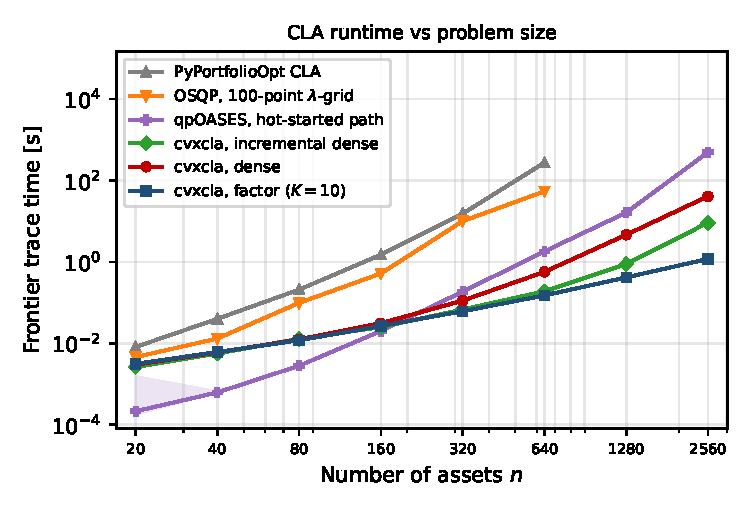
\includegraphics[width=0.54\textwidth]{scaling.pdf}
\caption{Frontier trace time against $n$ (log--log). Exponents $p$ of time $\approx n^p$,
fitted over the last four sizes each method was timed at with no overhead removed:
$2.9$ dense, $2.4$ incremental dense and $1.4$ factor ($n = 320$--$2560$), $3.4$
\pkg{PyPortfolioOpt} and $3.2$ \pkg{OSQP} ($80$--$640$), $3.7$ \pkg{qpOASES}
($320$--$2560$); they describe these sizes on this machine, not asymptotic complexity. \pkg{PyPortfolioOpt} and a warm-started \pkg{OSQP} grid of
$100$ values of $\lambda$ (\S\ref{sec:clarabel}) are timed up to $n=640$, and
\pkg{qpOASES} hot-started along the whole path (\S\ref{sec:qpoases}) up to $n=2560$.
The methods deliver different outputs: \pkg{cvxcla} and \pkg{PyPortfolioOpt} return
every turning point, the \pkg{OSQP} grid $100$ portfolios, and \pkg{qpOASES} only the
minimum-variance endpoint, so its time covers the path following alone.}
\label{fig:scaling}
\end{figure}

\subsection{Where the speed comes from}
\label{sec:baseline}

A fairer comparison sets \pkg{cvxcla}'s own dense backend against its opt-in
incremental one, \code{IncrementalDenseCovariance} (\S\ref{sec:incremental}), which runs the same loop
but maintains $\Sig_{\F\F}\inv$ by rank-one updates and reports the same turning points.
A trace is then $O(n^3)$, the measured exponent $\approx 2.4$, and the incremental
backend is about $3\times$ faster than the dense one at $n=640$ and $4.5\times$ at
$n=2560$: block elimination is not the fastest dense strategy. The factor backend is
still about $1.3\times$ faster than the incremental one at $n=640$ and $8\times$ at
$n=2560$, so the speed comes from the structured solve. Updating the Woodbury
capacitance $W$ incrementally would add little at $K=10$, where the $O(n)$ work of each
step (event scan, products with $\Sig$, bookkeeping) dominates, and matters only at
large $K$, where the dense backend is already faster (\S\ref{sec:rankscaling}).

\subsection{Runtime versus factor rank}
\label{sec:rankscaling}

The factor backend's advantage must fade as $K$ approaches $n$. At fixed $n = 320$ and
$K \in \{20, \dots, 320\}$ (\target{rank-scaling}), the dense time is flat in $K$ while Woodbury grows as
$O(n_\F K^2 + K^3)$: the factor backend is about $1.8\times$ faster at $K=20$, at parity near
$K=160$, and $\approx 1.7\times$ slower at $K = 320$. It pays off
in the regime real risk models inhabit, a few tens of factors over hundreds or thousands
of assets.

\subsection[A general-solver baseline: a QP swept over lambda]{A general-solver baseline: a QP swept over $\lambda$}
\label{sec:clarabel}

General toolkits (\pkg{Riskfolio-Lib} \citep{riskfolio}, \pkg{skfolio}
\citep{skfolio}, \pkg{fPortfolio} \citep{fportfolio}, \pkg{CVXR} \citep{cvxr}) hand a
single risk target to a general solver, so a frontier means re-solving \eqref{eq:qp} on
a grid. We make the grid as favourable as we can: \pkg{OSQP} \citep{stellato2020} is
set up once, each $\lambda$ changes only the linear term, and each solve warm-starts
from the last, over a fixed grid of $100$ values (\target{scaling}). The sweep grows
like $\approx n^{3.2}$ and is slower at every size, from about $1.5\times$ the dense
trace at $n=20$ to about $95\times$ at $n=640$ ($54$~s against $0.6$~s). On the
real frontier of \S\ref{sec:empirical} it is about $240\times$ slower at tolerance $10^{-6}$, and
at $10^{-5}$ it misses points by $10^{-3}$ (\target{osqp}). For a
single risk target a general solver is the natural choice; for the whole frontier on a
structured covariance, the trace is what separates \pkg{cvxcla} from these toolkits.

\subsection{A parametric QP solver}
\label{sec:qpoases}

\pkg{qpOASES} \citep{ferreau2014} solves parametric QPs by an online active-set
strategy: a hot start from one QP to the next follows the homotopy between them and
changes the working set at every breakpoint on the way. Hot-started from the
maximum-return end to $\lambda = 0$, it walks the same path as the CLA. We run it
through \pkg{CasADi} \citep{andersson2019}, solving once above the first finite turning
point and hot-starting once to $\lambda = 0$ (\target{scaling}).

The two codes follow the same path: \pkg{qpOASES} makes exactly as many working-set
changes as \pkg{cvxcla} reports turning points ($21, 42, \dots, 2561$), and its endpoint
matches the minimum-variance portfolio to $\sim\!2\times10^{-16}$. On small problems it
is faster, by a factor of several up to
$n=80$, where \pkg{cvxcla}'s \proglang{Python} per-step overhead dominates; the two meet
near $n=200$. Beyond that \pkg{qpOASES} grows like $\approx n^{3.7}$ and takes about $1.8$~s at
$n=640$ and $490$~s at $n=2560$: about $3\times$ and $12\times$ the dense backend, $12\times$
and $420\times$ the factor backend. It also returns only the endpoint, since the
turning points it passes are not exposed through the CasADi interface.

\subsection[Empirical example: the SP 500 frontier]{Empirical example: the S\&P 500 frontier}
\label{sec:empirical}

The experiment runs off a frozen snapshot shipped with the package:
$N = 494$ assets over $T = 1213$ trading days, 2021-07-30 to 2026-05-29, stored as
\srcfile{experiments/data/sp500_pct_returns.parquet}{sp500\_pct\_returns.parquet}
(SHA-256 \texttt{b5faa522\ldots9937e}) and produced once by
\srcfile{experiments/fetch_sp500.py}{fetch\_sp500.py}, retained for provenance only.
That script takes the index constituents listed on the day it was run, downloads their
split- and dividend-adjusted closes from \pkg{yfinance}, drops names missing more than
$5\%$ of the trading days, and forward-fills short gaps. The universe is the index at the end of the window, with survivorship bias, so we use it
only as a realistic covariance; it says nothing about investment performance. From the
full-history sample moments (condition number $\approx 1.1\times 10^{5}$) the CLA
traces the long-only frontier, $96$ turning points, in about $23$~ms;
a rank-$20$ factor approximation traces a
near-identical frontier ($89$ points) in about $15$~ms. The frontier spans annualised
returns of $0.14$--$0.89$ over volatilities of $0.10$--$0.87$, with an in-sample maximum
Sharpe ratio near $2.7$ (\target{real-frontier}).

\paragraph{Covariance estimators as backends.}
\label{sec:estimators}
Because \pkg{cvxcla} traces the frontier of whatever covariance it is given, a shrinkage
or factor estimate is simply another backend. Most remedies for a noisy sample
covariance \citep{johnstone2001} return the diagonal-plus-low-rank form
\eqref{eq:factor}: approximate factor models \citep{chamberlain1983}, POET
\citep{fan2013poet}, eigenvalue clipping \citep{laloux1999}, or Ledoit--Wolf shrinkage
\citep{ledoitwolf2004}, $(1-\rho)S + \rho F$. On the same universe, changing only the
covariance argument, \pkg{cvxcla} traces the frontier of the sample covariance ($96$
turning points), the Ledoit--Wolf estimate ($94$) and a rank-$20$ PCA model ($89$); the
three maximum-Sharpe portfolios hold $26$--$29$ names (\target{estimators}). As the
window shrinks past $T = n$ the sample covariance loses rank while the shrinkage and
factor estimates stay well-conditioned (\S\ref{sec:regularization}). \pkg{cvxcla}
controls only the computational error; an exact frontier of a noisy estimate is still
noisy, and ranking the estimators would take an out-of-sample study.


\section{Conclusion}

The Critical Line Algorithm computes the whole mean--variance frontier by walking its
piecewise-linear path from the maximum-return to the minimum-variance portfolio.
\pkg{cvxcla} takes each step with one block-eliminated KKT solve, resolves ties by a
least-index rule under which the walk provably terminates (Proposition~\ref{prop:termination}),
and reaches the covariance only through a five-member operator protocol. A factor risk
model therefore yields the same turning points as the dense matrix it represents; with $2560$ assets and ten factors it does so about $35$ times faster, in under $1$~MiB of working memory beyond the stored frontier. The gain is one of scale and structure. Below about $200$
assets the per-step overhead of \proglang{Python} dominates, and \pkg{qpOASES}, which
follows the same path, is faster.

\section*{Computational details}
\addcontentsline{toc}{section}{Computational details}

The results in this paper were obtained with \pkg{cvxcla}~2.6.0 \citep{cvxcla}, whose Critical Line Algorithm is unchanged in release~2.7.0, and
\proglang{Python}~3.14.6 on an Apple M4 Pro (14 cores, 48~GB of memory) under
macOS~15.6.1. \pkg{NumPy}~2.4.6 and \pkg{SciPy}~1.17.1 were linked against Apple's
Accelerate BLAS, and the first turning point under a general equality system is found
with the HiGHS solver through \code{scipy.optimize.linprog}. The comparisons use
\pkg{PyPortfolioOpt}~1.6.0, \pkg{OSQP}~1.1.3, and the \pkg{qpOASES} bundled with
\pkg{CasADi}~3.8.1. The estimators of \S\ref{sec:estimators} use
\pkg{scikit-learn}~1.9.0, the figures \pkg{matplotlib}~3.11.0, and the return data are
read with \pkg{pandas}~3.0.3 and \pkg{pyarrow}~24.0.0.

\paragraph{Software availability.}
\pkg{cvxcla} is released under the MIT license. Release~2.7.0, which ships the experiment script in the form used here, is
archived on Zenodo \citep{cvxcla} with DOI \textbf{[TODO: the Zenodo DOI of this release]}; the source is
developed at \url{https://github.com/cvxgrp/cvxcla}, and every source link in this paper
points to the release tag \code{v2.7.0}. The package declares only lower bounds on its
dependencies, and its continuous integration also tests them at those bounds; the
experiment script pins the exact versions above. The test suite, some $570$ unit and
property-based tests (the latter with \pkg{Hypothesis}), enforces full line coverage of
the library.

\paragraph{Reproducing the results.}
Every figure, table, and number is produced by one script,
\srcfile{experiments/make_figures.py}{make\_figures.py} in the \pkg{cvxcla} repository.
It declares the versions above as inline (PEP~723) metadata, so with \pkg{uv} installed
\begin{CodeInput}
uv run experiments/make_figures.py all
\end{CodeInput}
installs them into an isolated environment and rebuilds everything. A target name in
place of \code{all} rebuilds one artefact, and \code{all -{}-quick} skips the two scaling
sweeps (\S\ref{sec:scaling} and \S\ref{sec:rankscaling}), which take about $40$ minutes
on the machine above. Random inputs are drawn from fixed seeds and the S\&P 500 returns
are a committed snapshot (\S\ref{sec:empirical}), so the run needs no network access
once the packages are installed. Timings and memory were measured on this machine only and will differ elsewhere; the
turning-point counts and accuracy figures should agree up to round-off.

\section*{Acknowledgements}
\addcontentsline{toc}{section}{Acknowledgements}

The author thanks Stephen Boyd, Trevor Hastie and Philipp Schiele. The first versions of the
solver were implemented while the author stayed for a sabbatical at Boyd's group
at Stanford University.


\appendix
\section{Implementation details}
\label{sec:details}

\subsection{The event guards}
\label{sec:guards}

Slopes are tested against a floor of $\sqrt{\varepsilon_{\text{mach}}}$ in the
problem's own units, not against the user tolerance, which would let a tiny but genuine
slope go unnoticed. With $m = \lVert\mu\rVert_\infty$ and
$\sigma = \lVert\Sig\mathbf{1}\rVert_\infty/n$, $\lambda$ has the scale $\sigma/m$.
Weight slopes $\beta_i$ and slack slopes $g_j\trans\beta$ carry units of $1/\lambda$
and are tested against $\sqrt{\varepsilon_{\text{mach}}}\,m/\sigma$; multiplier slopes
$\delta_i$, $\eta^{\beta}_j$ carry the units of $\mu$ and are tested against
$\sqrt{\varepsilon_{\text{mach}}}\,m$. The $\lambda$ window is a relative $10^{-10}$
taken against $\max(\lvert\lambda\rvert, \sigma/m)$, so that it does not vanish as
$\lambda \to 0$.

\label{sec:invariance}\label{sec:moreexp}%
The trace does not depend on the units (\target{validate-scaling}). Rescaling the returns
by $c$ and the covariance by $s$, each from $10^{-6}$ to $10^{6}$, leaves all $29$
turning points of the $40$-asset problem in place: the weights agree to
$8\times10^{-15}$, and $\lambda c/s$ to a relative $1.2\times10^{-13}$. Multiplying the
slope floors by any factor from $10^{-6}$ to $10^{4}$ leaves the traces of the $40$- and
$494$-asset S\&P 500 problems, the $600$-day window and the $320$-asset factor market bit
for bit unchanged. Only at $10^{6}$ does the floor start to swallow genuine slopes: the
$40$-asset trace is still unchanged, the $600$-day window's weights move by
$7\times10^{-2}$, and the trace of the $494$-asset problem and of the factor market is
declined. So on these inputs genuine slopes and round-off are about ten orders of
magnitude apart. A turning point
lost to the floor would leave the later ones feasible but not optimal, which the KKT
certificate reports as a stationarity or dual-feasibility residual.

\subsection{The gross-exposure lift}
\label{sec:liftdetail}

Both legs of an asset are never free together on the path. Write $g_i$ for the $i$-th
entry of $\Sig w - \lambda\mu + A\trans\nu + G\trans\eta_G$ and $\eta\ge 0$ for the
multiplier of the cap; the reduced gradients of the two legs are $g_i + \eta$ and
$-g_i + \eta$. A free long leg has $g_i = -\eta$, so its short leg's reduced gradient
is $2\eta$; a long leg at its upper bound has $g_i + \eta \le 0$, so its short leg's is
at least $2\eta$ (and symmetrically). The idle leg can therefore enter only where $\eta$
vanishes, at the release of the cap, and the event search drops that competing leg
event so the release fires.

At the first vertex, overlapping legs (the cap tight with a zero multiplier) are removed
by subtracting $\min(x_i^+, x_i^-)$ from both, which leaves $w$ and every other
constraint unchanged; a cap at the smallest feasible gross exposure ($c = 1$ under a
full budget), which fails Slater's condition, is handled by solving
$\min \mathbf{1}\trans x$ first and pinning every leg with a positive reduced cost.

\subsection{The degenerate first vertex}
\label{sec:vertexdetail}

The maximum-return vertex can be degenerate: every weight on a bound (any inequality row on a
long-only problem whose best asset takes the whole budget), or a duplicated tight row.
Its partition is then read off the linear program's duals, generalising the budget rule
of \S\ref{sec:first}. At a degenerate vertex these are not unique, and the solution the simplex
reports can show too few zero reduced costs to free enough assets. For example, with
three assets, $\mu = (3, 2, 1)$, long-only, the budget and the row $w_2 = 0$, HiGHS
reports duals that free only the first asset at $w = (1, 0, 0)$, whereas the equally
optimal multipliers $1$ on both rows free the other two. The code therefore first moves
the reported duals to a vertex of the optimal dual set, stepping along directions that
keep the tight dual constraints tight until they determine the multipliers. A basis is
read off that dual vertex: the assets strictly inside their bounds, then the tight rows
with zero multiplier, which are released, then the assets on a bound with zero reduced
cost, in order of decreasing return, which are freed. The active rows then have a square,
nonsingular free block, the first segment starts at the vertex itself, and the implied
multipliers are those of the dual vertex, so the partition is dual feasible. The optimal
dual set has no vertex, and the vertex is refused, when a tight row touches only assets
fixed at both bounds.

Nearly dependent equality rows, such as $\mathbf{1}\trans w = 1$ and
$(\mathbf{1} + \epsilon v)\trans w = 1$, which encode $v\trans w = 0$ only at scale
$\epsilon$, would be enforced by the linear program only to its tolerance divided by
$\epsilon$. When the row-normalised equality matrix has a reciprocal condition number
below $10^{-6}$ they are handed to HiGHS in orthonormal rows, $Q\trans w = R^{-\mathsf{T}}
b$ with $A\trans = QR$.

\section{Numerical robustness: degeneracy and ties}
\label{sec:degeneracy}

\paragraph{Round-off.}
A candidate turning point can be optimal to solver precision but not exactly feasible:
round-off accumulated over hundreds of turning points can leave a free weight a hair
outside its box. \code{CLA.\_emit} projects such a point back onto the feasible set
before it validates it. The projection is a numerical repair: it keeps the point
optimal to working accuracy only when the correction is small and lies in near-flat
directions of the objective, where round-off usually sits, so we measure it below. For the plain budget with no active inequality row the projection
onto the capped simplex is closed-form (a single shift, found by bisection, then a
clip). Under a general $A$ or an active row of $G$
the code alternates a box clip with the affine projection onto $\{w : C w = c\}$,
$C = [\,A;\,G_{\Sset}\,]$, written in orthonormal rows so that its Gram matrix is the
identity rather than $CC\trans$. It usually converges in one iteration, stops once the box is violated by at most
$10^{-12}$, and raises a \code{ProjectionError} if $100$ iterations do not get there.

The measurements of \target{validate-projection} support this for the problems tested.
On the rank-deficiency sweep of Figure~\ref{fig:degeneracy} and the S\&P 500 windows of
\S\ref{sec:estimators}, the projection changes between none and four turning points per
trace; the largest weight correction is $9.3\times10^{-15}$, the largest relative change
of the objective $8.7\times10^{-19}$, and every projected point satisfies the box and the
budget to $2.2\times10^{-16}$. The KKT certificate (Table~\ref{tab:kkt}) bounds every
residual on the segments between projected points by $2\times10^{-13}$, and every
completed trace of the sweep matches a reference QP in objective to $\sim\!10^{-13}$.

\paragraph{Rank deficiency.}
The two regimes are told apart by the \emph{conditioning} of the free block. While it
stays numerically full rank any infeasibility is round-off and is projected away. Once
the free set outgrows the covariance rank, $\Sig_{\F\F}$ is singular, but the reduced
system \eqref{eq:kkt} need not be: the active rows $C_\F$ hold the free weights on their
null space, and the system is uniquely solvable when $Z\trans\Sig_{\F\F}Z$ is positive
definite, where the columns of $Z$ span $\{v : C_\F v = 0\}$. A guard reads the
reciprocal condition number of $\Sig_{\F\F}$ from its eigenvalues, a quantity that,
unlike the size of a violation, is stable across BLAS builds. When it falls below
$10^{-12}$ the guard reads that of $Z\trans\Sig_{\F\F}Z$ instead, the segment is solved
on the null space, and the trace is declined with a diagnosis only when that block is
singular too, since projecting its output could silently yield a suboptimal frontier.
Releases up to 2.5.0 declined as soon as $\Sig_{\F\F}$ was singular, which refused the
frontier of a sample covariance from fewer observations than assets whenever its free
set outgrew the data rank (\target{degeneracy}). Singular constraint rows, at the first vertex or later in the
trace, are declined in the same way (\S\ref{sec:first}, \S\ref{sec:ineq}).

\begin{figure}[t]
\centering
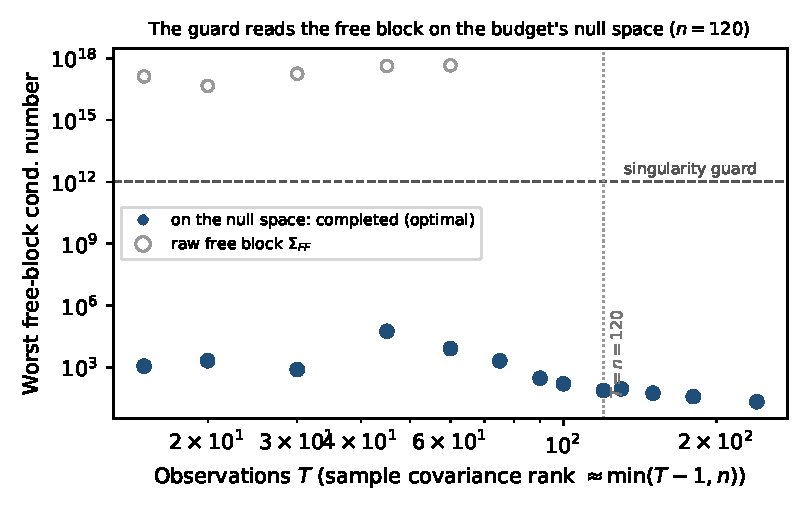
\includegraphics[width=0.5\textwidth]{degeneracy.pdf}
\caption{A rank-deficiency sweep at $n = 120$, the long-only covariance estimated from
$T$ observations. Grey rings are the worst condition number of the raw free block
$\Sig_{\F\F}$ over a trace; blue circles that of $Z\trans\Sig_{\F\F}Z$, the block on the
budget's null space, which is what the guard (dashed, $10^{12}$) reads. Below $T = 75$
the raw block is singular ($\sim\!10^{17}$) while the reduced block stays below
$6\times10^{4}$, so every trace completes, and every completed frontier matches a
reference QP to $3\times10^{-13}$. Release~2.3.3 declined the five windows with
$T \le 60$.}
\label{fig:degeneracy}
\end{figure}

\paragraph{Conditioning.}
To see the guard on its own we prescribe the spectrum,
$\Sig = Q \operatorname{diag}(\lambda) Q^\top$ with $60$ eigenvalues spread geometrically
from $1$ to $1/\kappa$, under a long-only budget, and certify each trace
(\target{validate-conditioning}). With a random orthogonal
$Q$ the free blocks see only part of the spectrum, their worst condition number stays at
$5.9\times10^{9}$ for $\kappa = 10^{16}$, and every trace completes with KKT residuals
below $2.5\times10^{-14}$. With $Q = I$ the free block inherits the full spread: traces
up to $\kappa = 10^{12}$ complete and are certified (residuals up to
$5.5\times10^{-12}$), and from $3\times10^{12}$ to $10^{14}$ every trace is declined at
the guard, so here its value decides the outcome. At $\kappa = 10^{16}$ the smallest
eigenvalues are zero to working precision; the trace completes again, in $10$ turning
points, and is certified ($3.9\times10^{-15}$). It and \pkg{OSQP} reach different weights,
up to $0.94$ apart, yet both meet the optimality conditions, so there the optimum is not
unique.

The reference QP is the less accurate of the two: OSQP leaves KKT residuals near
$10^{-9}$ and differs from the trace by up to $0.2$ in a weight in the diagonal family,
where the KKT conditions only weakly determine the weights along directions of tiny
variance. None of the $192$ reference solves failed.

\paragraph{Event ties.}
Ties are handled by the least-index rule of \S\ref{sec:bland}. Across four deliberately
degenerate families of $32$ instances each ($n$ up to $240$; \target{tie-degeneracy}),
a trace counts only if it is optimal: every turning point must pass the KKT certificate
of Table~\ref{tab:kkt} to $10^{-8}$, so a frontier that ends but is wrong is reported
as such. Exactly tied means give $31$ certified traces; the other instance ($n=60$) is
declined partway along the frontier, at a degenerate turning point whose multipliers are
not unique. Exchangeable pairs (identical means and covariance rows) give $32$ certified
traces, and the tie-break never frees both members of a pair. A family of
$p\approx n/3$ group caps gives $32$, with up to $53$ rows active at once, and an
over-constrained family of $p=n$ overlapping caps, whose maximum-return vertex is
degenerate, gives $32$, with up to $240$ rows active at once. No trace is off the
frontier.

\paragraph{A correction.}
The first version of this paper, run with release~2.3.3, counted completions without
certifying them, and reported that the tied-means and exchangeable families all
complete. They did complete, but none is on the efficient frontier: certified, all $32$
tied-means and all $32$ exchangeable traces of 2.3.3 fail the certificate, and on the
tied-means family with $n\le120$ their objective exceeds that of an interior-point
solve by up to a factor of $26$. Both families share
the largest expected return between several assets, and 2.3.3 started such a frontier
at an arbitrary vertex of the tied face (\S\ref{sec:first}). The group-cap family was
right, and $30$ of the $32$ overlapping-cap traces were, the other two declined.

The tied-means and group-cap families, the full-rank windows of
Figure~\ref{fig:degeneracy} and both conditioning families satisfy the hypotheses of
Proposition~\ref{prop:termination} at every turning point, so for them termination is
the theorem. The others do not. In the exchangeable family all $1751$ tied turning
points satisfy the hypotheses. The overlapping-cap traces pass $2637$ ties, all with
dependent constraints, so for them only the weaker guarantees of \S\ref{sec:bland} hold.
The nine rank-deficient windows of Figure~\ref{fig:degeneracy} have a singular $\Sig$,
outside $\Sig\succ0$; all nine complete, the five with $T\le 60$ by solving on the
budget's null space. No trace used more than $1.5\%$ of the iteration cap
$100(n+p+1)$.

\section[Relation to other CLA implementations]{Relation to other CLA implementations}
\label{sec:baileydetail}

The most widely used open CLA is that of \citet{bailey2013}, behind
\pkg{PyPortfolioOpt}'s \code{CLA}. It shares the greedy first turning point and the
explicit minimum-variance endpoint of \pkg{cvxcla} and aims at the same turning points,
but it is built without the Karush--Kuhn--Tucker conditions. \citet[p.~173]{bailey2013}
name them as one option for the inequality-constrained problem and instead ``divide and
conquer'' it into unconstrained problems on the free assets. Without multipliers on the
bounds, deciding which blocked asset to free takes a fresh inverse of the free block for
every candidate, each inserted into closed-form Lagrange expressions for one budget row;
in \pkg{cvxcla} the same decision is the sign of $\gamma_i + \lambda\delta_i$ from a single
solve (\S\ref{sec:events}). Their code then removes turning points that violate the
bounds or the convex hull after the fact (\code{purgeNumErr}, \code{purgeExcess});
\pkg{cvxcla} checks the same conditions with a KKT certificate (\S\ref{sec:exactness}).
In \pkg{PyPortfolioOpt}~1.6.0 those violations are not round-off: after a weight leaves
the free set, the next turning point is solved with that weight's previous value rather
than its bound, so it misses the budget and is purged; \code{purgeExcess} compares
expected returns without a tolerance. Both delete genuine turning points.
Ties are broken by a strict comparison, with no anti-cycling rule. On the scaling problems of \S\ref{sec:scaling}
\pkg{PyPortfolioOpt}'s corners are a subset of \pkg{cvxcla}'s
($19, 42, 81, 158, 323, 641$ against $21, 42, 81, 159, 323, 641$). The missing corners are
genuine, so across them its frontier is wrong, by up to $7\times10^{-3}$ in a weight at
$n=20$ and $8\times10^{-5}$ at $n=160$; at the other sizes the two frontiers agree to
$10^{-12}$, and the minimum-variance endpoints to $\sim\!10^{-16}$ throughout. Reading the
blocked weights from the current iterate and comparing with a tolerance removes the
discrepancy.

Written with the KKT conditions, the method is also the shorter one:
Figure~\ref{fig:kktcla} is a complete CLA for the problem class of \citet{bailey2013} in
39 lines of \pkg{NumPy}, against about $180$ for the trace in \pkg{PyPortfolioOpt}. Each
segment costs one bordered solve of \eqref{eq:saddle}, every event is read off it
(\S\ref{sec:events}), and events are compared with a relative tolerance. On the scaling
problems of \S\ref{sec:scaling} it returns \pkg{cvxcla}'s turning points to $10^{-13}$, in
time of the same order as the dense backend. It refuses rather than mis-solves infeasible
bounds, a tied largest return (\S\ref{sec:first}) and a singular free block
(Appendix~\ref{sec:degeneracy}); \pkg{cvxcla} handles the last two.

\begin{figure}[!ht]
\begin{lstlisting}[style=pyin,basicstyle=\ttfamily\footnotesize]
import numpy as np

def cla(mu, S, lo, up, tol=1e-9):
    """Turning points (lam, w) of max lam mu'w - w'Sw/2, 1'w=1, lo<=w<=up."""
    n, w, rest = len(mu), lo.astype(float), 1.0 - lo.sum()
    for i in np.argsort(-mu, kind="stable"):   # first turning point
        take = min(up[i] - lo[i], rest)
        w[i], rest = w[i] + take, rest - take
        if rest <= 0:
            break
    if rest > 0 or (n > 1 and np.partition(mu, -2)[-2] == mu.max()):
        raise ValueError("infeasible bounds, or a tied largest return")
    F, lam, last, path = np.arange(n) == i, np.inf, -1, [(np.inf, w.copy())]
    while True:                                # one KKT solve per segment
        B, m, one = ~F, F.sum(), np.ones(F.sum())
        K = np.block([[S[np.ix_(F, F)], one[:, None]], [one, 0.0]])
        rhs = np.c_[np.r_[-S[np.ix_(F, B)] @ w[B], 1 - w[B].sum()],
                    np.r_[mu[F], 0.0]]
        x = np.linalg.solve(K, rhs)            # w_F = a + lam b, nu likewise
        a, b = w.copy(), np.zeros(n)
        a[F], b[F] = x[:m, 0], x[:m, 1]
        gam, dlt = S @ a + x[m, 0], S @ b - mu + x[m, 1]  # reduced cost
        with np.errstate(divide="ignore", invalid="ignore"):
            hit = np.where(F, np.where(b < 0, up - a, lo - a) / b, -gam / dlt)
        live = np.where(F, abs(b) > tol,
                        np.where(w <= lo, dlt > tol, dlt < -tol) & (lo < up))
        if last >= 0:
            live[last] = False                 # the asset that just flipped
        hit = np.where(live & (hit <= lam * (1 + tol)), hit, -np.inf)
        k = int(np.argmax(hit))                # ties: lowest index
        if hit[k] <= 0:
            return [*path, (0.0, a)]
        lam, w = hit[k], a + hit[k] * b
        if np.any((w < lo - 1e-8) | (w > up + 1e-8)):
            raise np.linalg.LinAlgError("free block numerically singular")
        if F[k]:
            w[k] = up[k] if b[k] < 0 else lo[k]  # leaving weight on its bound
        F[k], last = not F[k], k
        path.append((lam, w.copy()))
\end{lstlisting}
\caption{A complete CLA for box bounds and one budget row, written with the KKT conditions.}
\label{fig:kktcla}
\end{figure}

The large-scale active-set methods of \citet{perold1984}, \citet{stein2008} and
\citet{hirschberger2010} cut the per-step cost through incremental factorisations,
sparsity or pivoting tied to an explicit matrix; we could not run their codes or that of
\citet{niedermayer2010} on current toolchains, and compare instead with \pkg{qpOASES}
(\S\ref{sec:qpoases}).

\section[Proof of the termination proposition]{Proof of Proposition~\ref{prop:termination}}
\label{sec:proof}

\paragraph{Leaving is permanent.}
A partition (free set, blocked bounds, active rows $\Sset$) is valid at $\lambda$ when
its segment respects the bounds and the inactive rows and its multipliers have the right
signs. Each of these conditions is affine in $\lambda$. An event fires at
$\lambda^{\star}$ because one of them is zero there with a slope that violates it below
$\lambda^{\star}$ (the slope floor makes every event a strict crossing), and an affine
function that crosses zero stays on the wrong side, so a partition left at
$\lambda^{\star}$ is invalid at every $\lambda < \lambda^{\star}$. Since $\lambda$ never
increases, a partition can recur only at the same $\lambda^{\star}$, within a tie.

\paragraph{The direction problem at a tie.}
Fix $\lambda^{\star}$. Because $\Sig \succ 0$ the optimiser
$w^{\star} = w(\lambda^{\star})$ is unique, and by linear independence so are its
multipliers. Constraints with slack, or holding with a nonzero multiplier, cannot fire
at $\lambda^{\star}$, and every partition the walk visits there keeps their status; let
$E$ stack the gradients of the latter together with $A$. The partitions differ only on
the set $T$ of tied constraints, those holding with a zero multiplier, written
$c_t\trans w \le \text{const}$ (with $c_t = \pm e_i$ for a bound). Below $\lambda^{\star}$
the walk follows a segment $w(\lambda^{\star} - \tau) = w^{\star} + \tau d$, $d = -\beta$,
on which the multipliers are affine in $\tau$ too, $\nu(\tau) = \nu^{\star} + \tau\nu'$.
Substitute both into the KKT conditions of \eqref{eq:qp} and keep the terms of order
$\tau$. Stationarity gives $\Sig d + \mu + E\trans \nu'_E + C_T\trans \nu'_T = 0$. A
constraint in $E$ keeps a nonzero multiplier for small $\tau$, so it stays active and
$E d = 0$. A tied constraint has slack $-\tau\, c_t\trans d$ and multiplier
$\tau\,\nu'_t$, so feasibility, the sign of the multiplier, and complementary slackness
require $c_t\trans d \le 0$, $\nu'_t \ge 0$, and $(c_t\trans d)\,\nu'_t = 0$. These are
the KKT conditions of the strictly convex QP
\[
\min_d\; \tfrac12\, d\trans \Sig d + \mu\trans d
\quad\text{subject to}\quad E d = 0,\quad c_t\trans d \le 0 \;\; (t \in T),
\]
so $d$ is its unique solution, the classical directional derivative of a parametric
program without strict complementarity \citep{jittorntrum1984, bonnans2000}.

\paragraph{The complementarity problem.}
Let $E$ have linearly independent rows, let $Z$ be a basis of its null space, and let
$C_T$ collect the columns $c_t$, $t \in T$. Every $d$ with $Ed = 0$ is $d = Zy$, and the
direction problem becomes $\min_y \tfrac12\, y\trans H y + \mu\trans Z y$ subject to
$C_T\trans Z y \le 0$, with $H = Z\trans \Sig Z \succ 0$ because $\Sig \succ 0$ and $Z$
has full column rank. Its KKT conditions, with slacks $s = -C_T\trans Z y$ and
multipliers $\nu \ge 0$, eliminate $y = -H\inv Z\trans(\mu + C_T \nu)$ and leave the
linear complementarity problem
\[
s = q + M\nu, \qquad s \ge 0,\; \nu \ge 0,\; s\trans\nu = 0, \qquad
M = C_T\trans Z H\inv Z\trans C_T,\quad q = C_T\trans Z H\inv Z\trans \mu .
\]
$M$ is positive semidefinite, and positive definite exactly when $Z\trans C_T$ has full
column rank. Suppose $Z\trans C_T\, x = 0$. Then $C_T x$ lies in the null space of
$Z\trans$, which is the row space of $E$, so $C_T x = E\trans z$ for some $z$, and
$[\,E\trans,\ C_T\,]\,(-z, x) = 0$. The hypothesis that the gradients of $E$ and of the
tied constraints are linearly independent forces $z = 0$ and $x = 0$. Hence $M \succ 0$,
and in particular $M$ is a P-matrix: every principal minor is positive.

\paragraph{The correspondence with the implementation.}
Each tied constraint $t$ contributes one complementary pair $(s_t, \nu_t)$, and a
partition visited at $\lambda^{\star}$ makes exactly one of the two basic: $s_t$ when the
constraint is released (a free weight, an inactive row), $\nu_t$ when it is enforced (a
blocked weight, an active row). The $\beta$-system of that partition
(\S\ref{sec:blockelim}) is the equality-constrained form of the direction problem with
the enforced constraints held, so its solution is the basic solution of the
complementarity problem. Table~\ref{tab:pivots} lists the six event types of the code
(\srcfile{src/cvxcla/_events.py}{\_events.py}). Each fires at $\lambda^{\star}$ exactly
when the basic variable of its pair is negative: a released constraint whose slack would
turn negative as $\lambda$ falls, or an enforced one whose multiplier would.

\begin{table}[t]
\centering
\small
\begin{tabular}{llll}
\hline
Event (column) & Status of $t$ & Basic variable & Fires at $\lambda^{\star}$ when \\
\hline
free weight reaches its upper bound (0) & released & $s_t$ & $\beta_i < 0$ \\
free weight reaches its lower bound (1) & released & $s_t$ & $\beta_i > 0$ \\
blocked weight leaves its upper bound (2) & enforced & $\nu_t$ & $\delta_i < 0$ \\
blocked weight leaves its lower bound (3) & enforced & $\nu_t$ & $\delta_i > 0$ \\
inactive row binds (0, row block) & released & $s_t$ & $g_j\trans\beta < 0$ \\
active row releases (1, row block) & enforced & $\nu_t$ & $\eta^{\beta}_j > 0$ \\
\hline
\end{tabular}
\caption{The six event types of the event scan and the complementary pair each one
pivots. A coordinate's status admits one event type at a time, so a coordinate index
identifies the pair.}
\label{tab:pivots}
\end{table}

\paragraph{The pivoting rule.}
When several events fire at $\lambda^{\star}$, \code{select\_next\_event}
(\srcfile{src/cvxcla/pathtracer.py}{pathtracer.py}) flips the one with the lowest
coordinate index, assets before inequality rows, and changes the status of that
coordinate alone. By the correspondence above this is a simple principal pivot on the
lowest-index pair whose basic variable is negative, in a fixed ordering of the pairs:
Murty's least-index method \citep{murty1974}, which terminates on every linear
complementarity problem with a P-matrix, for every $q$ \citep{murty1974, cottle1992}.
The pivot depends only on the current partition, so a partition repeated at
$\lambda^{\star}$ would repeat forever; none is, and the walk leaves $\lambda^{\star}$ after
finitely many steps with a feasible basic solution, along a segment of positive length.

\paragraph{Termination.}
Each segment of positive length uses a partition never used before, and there are
finitely many partitions; each tie between two such segments takes finitely many steps.


\bibliography{refs/references}

\end{document}
